\documentclass[a4paper, 11pt]{article}
\usepackage{marginnote}


\def\nterm {Spring}
\def\nyear {2023}
\def\nlecturer {Carlos Améndola}
\def\ncourse {Discrete Geometry III}

\ifx \nlecturer\undefined 
	\author{Notes taken by Viet Duc Nguyen}
\else
	\author{Based on lectures by \nlecturer}
\fi
\date{\nterm\ \nyear}
\title{\ncourse}

\usepackage[utf8]{inputenc}
\usepackage{amsmath,amsthm,amssymb}
\makeatletter
\def\th@plain{%
  \thm@notefont{}% same as heading font
  \itshape % body font
}
\def\th@definition{%
  \thm@notefont{}% same as heading font
  \normalfont % body font
}
\makeatother
\usepackage{mathtools}
\usepackage{bbm}
\usepackage{marvosym}
\usepackage{array}
\usepackage{geometry}
\usepackage[toc,titletoc,title]{appendix}
\usepackage[hidelinks]{hyperref}
\usepackage{framed}
\usepackage{caption}
\usepackage{subcaption}
\usepackage{enumitem}
\usepackage{tikz}
\usetikzlibrary{patterns}
\usetikzlibrary{shapes}
\usetikzlibrary{plotmarks}
\usetikzlibrary{cd}

\usepackage{float}
\usepackage{xcolor}
\hypersetup{
	colorlinks,
	linkcolor={red!50!black},
	citecolor={red!50!black},
	urlcolor={red!50!black}
}


\makeatletter
\let\@real@maketitle\maketitle
\renewcommand{\maketitle}{\@real@maketitle\begin{center}\begin{minipage}[c]{0.9\textwidth}\centering\footnotesize Updated on \date{\today}
 \\	These notes are not endorsed by the lecturer.\end{minipage}\end{center}}
\makeatother

\DeclareMathOperator*{\argmax}{arg\,max}
\DeclareMathOperator*{\argmin}{arg\,min}


\theoremstyle{definition}
\newtheorem{thm}{Theorem}[section]
\newtheorem{lemma}[thm]{Lemma}
\newtheorem*{lemma*}{Lemma}
\newtheorem{cor}[thm]{Corollary}
\newtheorem{prop}[thm]{Proposition}
\newtheorem{defi}[thm]{Definition}
\newtheorem{eg}[thm]{Example}
\newtheorem{remark}[thm]{Remark}
\newtheorem{ex}[thm]{Exercise}
\newtheorem{note}[thm]{Note}
\usepackage{makeidx}
\usepackage[]{mdframed}
\usepackage{algpseudocode}

\makeindex

\newcommand{\PhantC}{\phantom{\colon}}%
\newcommand{\PhantSQ}{\phantom{\sqrt{\hspace{0.3ex}}}}%
\newcommand*{\vertbar}{\rule[-1ex]{0.5pt}{2.5ex}}
\newcommand*{\horzbar}{\rule[.5ex]{2.5ex}{0.5pt}}

% https://tex.stackexchange.com/questions/63355/wrapping-cmidrule-in-a-macro
\ExplSyntaxOn
\makeatletter
\newcommand{\CMidRule}{\noalign\bgroup\@CMidRule{}}
\NewDocumentCommand{\@CMidRule}{
    m % Material to reinsert before cmidrule.
    O{0.0ex} % #1 = left adjust
    O{0.0ex} % #1 = right adjust
    m  %       #3 = columns to span
}{
    \peek_meaning_remove_ignore_spaces:NTF \CMidRule
      { \@CMidRule { #1 \cmidrule[\cmidrulewidth](l{#2}r{#3}){#4} } }
      { \egroup #1 \cmidrule[\cmidrulewidth](l{#2}r{#3}){#4} }
}
\makeatother
\ExplSyntaxOff


\begin{document}
\maketitle
\tableofcontents

\clearpage

\section{Gröbner basis}

\subsection{Monomial order}

\marginnote{\small{Lec01, 04/17/23}}

\begin{defi}[Poset]\index{poset}
  \( (A, \preceq) \) is called a {\textbf{poset}} if \( \preceq \) is 
  \begin{itemize}
    \item reflexive,
    \item anti-symmetric  (i.e. \( a \preceq b \) and \( b \preceq a \) imply \( a = b \)), and 
    \item transitive.
  \end{itemize}
\end{defi}

\begin{defi}[Well-order]
  A poset is called a \textbf{well-order}\index{poset} if every nonempty subset \( S \subset A \) has a minimum, i.e. there exists \( s \in S \) such that \( s \preceq s'  \) for all \( s' \in S \).
\end{defi}

\begin{remark}[well-order \( \implies \) total order]
  A well-order is a total order because for any \( a,b \in A \) the set \( \{ a,b \} \) has a minimum; hence \( a \preceq b \) or \( b \preceq a \).

  A total order need not be a well-order. As an example, take the integers \( \mathbb Z \) with the usual ordering \( \leq \).
\end{remark}

For a total order to be a well-order we need the \textbf{descending chain condition (DCC)}. DCC means that every descending chain \( \dots \preceq a_3 \preceq a_2 \preceq a_1 \) stabilizes.

\begin{prop}[total order + DCC = well-order]
  Let \( \preceq \) be a total order. Then, 
  \begin{align*}
    \preceq \text{ is well-order} \iff \preceq \text{ satisfies DCC}.
  \end{align*}
  Equivalently, infinite strictly descending chains \( \dots \prec a_3 \prec a_2 \prec a_1  \) do not exist.
\end{prop}

\begin{proof}
  \( \implies \) by contraposition. Assume there exists a non-terminating chain \( a_1 \preceq a_2 \preceq a_3 \preceq \dots \). Then, \( \left\{ a_i \right\}_{i \in \mathbb{N}} \) has no minimum.

  \( \impliedby \) by contraposition. Assume a nonempty subset has no minimum. Let \( a_0 \) be any element from the subset. Take \( a_i \) to be an element different from \( a_{i-1} \) such that \( a_i \preceq a_{i-1} \) by axiom of choice. We found a non-terminating descending chain.
\end{proof}

\begin{defi}[Admissable order]
  A poset \( (\mathbb N^n, \preceq) \) is called \textbf{admissable} if for all \( a,b,c \in \mathbb N^n \) we have \( a \preceq b  \implies a + c \preceq b + c  \).
\end{defi}

\begin{defi}[Polynomial]
  Let \( k \) be a field. A polynomial \( f \in k[x_1,\dots,x_n] \) is of the form \( f = \sum_{\alpha \in A} c_{\alpha} x^\alpha \), where \( A \subset \mathbb N^n \) is finite and \( c_\alpha \in k \). 
\end{defi}

\begin{defi}[Monomial order]\index{monomial order}
  A \textbf{monomial order} is an admissable, well-ordered and total order on \( \mathbb N^n \).
\end{defi}
It is called a monomial order because we define an ordering on monomials by 
\begin{align*}
  x^\alpha \prec x^\beta \iff \alpha \prec \beta.
\end{align*}

\begin{prop}[Monomial order respects \( \leq \)]
  Let \( \preceq \) be a monomial order and \( \alpha, \beta \in \mathbb N^n \). If \( \alpha \leq \beta \), then \( \alpha \preceq \beta \).
\end{prop}

\begin{proof}
  We have \( \alpha + \gamma = \beta \) for some \( \gamma \). Then, \( 0 \preceq x^\gamma \implies  \alpha \preceq \alpha + \gamma = \beta \).
\end{proof}


Checking if something is a well-order can be difficult. We have the following easy criterion for admissable total orderings. The proof is not trivial.

\begin{prop}[Easy criterion for well-order]
  Let \( \preceq \) be an admissable, total order on \( \mathbb N^n \). It is a well-order if and only if \(\mathbf 0 \preceq \mathbf x \) for all \( \mathbf x \in \mathbb N^n\).
\end{prop}

\begin{proof}\(  \)

  \( \implies \) by contraposition. Assume \(  \mathbf x \prec \mathbf 0 \). Then we found an infinite strictly decreasing chain \(\dots \prec 3 \mathbf x \prec 2 \mathbf x \prec \mathbf x \prec \mathbf 0\). Hence, DCC is not satisfied.

  \( \impliedby \) by induction on \( n \). For \( n = 1 \), \( \preceq \) must be the usual order \( \leq \) because we assume \( 0 \preceq 1 \). \( (\mathbb N, \leq) \) is clearly a well-order, so \( n=1 \) is done. For \( n \leadsto n+1 \), we define an order \( \prec' \) on \( \mathbb N^n \) by
    \begin{align*}
      \mathbf x \preceq' \mathbf y \iff  (\mathbf x,0) \preceq(\mathbf y,0) \qquad \mathbf x, \mathbf y \in \mathbb N^n.
    \end{align*}

  
  Let \( S \subset \mathbb N^{n+1} \) be nonempty and define the projection \( \pi: \mathbb N^{n+1} \to \mathbb N \) dropping the last coordinate. Set \( S' = \mathrm{im}(\pi) \subset \mathbb N^n \).
  
  By induction hypothesis, \( S' \) has a minimum \( \mathbf x' \) with respect to \( \preceq' \). Define \( \mathbf x \in S \) to be the element that projects to \( \mathbf x' \) and is minimal in the sense that \( \mathbf x_{n+1} \leq \mathbf y_{n+1} \) for all \( \mathbf y \in \pi^{-1}(\mathbf x') \). Define \( \ell = \mathbf x_{n+1} \). The following lemma shows that \( \mathbf x \) is minimal among all vectors in \( S \) that project to \( \mathbf x' \).
    
  \begin{lemma*}
    It holds: \( \mathbf x \preceq \mathbf y \) for all \( \mathbf y \in \pi^{-1}(\mathbf x') \).
  \end{lemma*}
  \begin{proof}
    We define \( \delta = \mathbf y_{n+ 1} - \ell \geq 0 \). By assumption, \( \mathbf 0 \prec  (\mathbf 0,\delta)  \). Adding \( (\mathbf x',\ell) \) we get \( (\mathbf x', \ell) \preceq (\mathbf x',\mathbf y_{n+1}) \). Hence, \( \mathbf x \preceq \mathbf y \).
  \end{proof}
  
  Continuing the proof, we set \( \mathbf x'^{(i)} = \min_{\prec'}\left\{ \mathbf z \in S' : (\mathbf z, i) \in S \right\} \) and \( \mathbf x^{(i)} = (\mathbf x'^{(i)}, i) \in S \) for \( i \in \left\{ 1,...,\ell - 1 \right\} \). Define 
  \begin{align*}
    \mathbf s = \min\left\{ \mathbf x^{(0)},\dots,\mathbf x^{(\ell-1)}, \mathbf x  \right\}.
  \end{align*}
  It is left to check that \( \mathbf s \) is the minimum of \( S \). We use the following lemma.

  \begin{lemma*}
    Assume \(  \mathbf v, \mathbf w \in \mathbb N^{n+1 } \) with \( \mathbf v_{n+1} = \mathbf w_{n+1} \). Then, 
    \begin{align*}
      \mathbf v \preceq \mathbf w \iff (\mathbf v_1,...,\mathbf v_n,0) \preceq (\mathbf w_1,...,\mathbf w_n,0).
    \end{align*}
  \end{lemma*}
  \begin{proof}
    \( \implies \) by contraposition: Assume \(   (\mathbf w_1,...,\mathbf w_n,0) \preceq (\mathbf v_1,...,\mathbf v_n,0) \). Add \( (\mathbf 0,\mathbf v_{n+1}) \) on both sides and we get \(\mathbf  w \preceq \mathbf v \). The converse direction \( \impliedby \) is similar.
  \end{proof}
  With this lemma, it is easy to show that \( \mathbf s \) is the minimum of \( S \).  Assume \( \mathbf y  \in S \). 
  
  If \( \mathbf y_{n+1} = \ell \), then the previous lemma implies \( \mathbf x \preceq \mathbf y \). 
  
  If \( \mathbf y_{n+1} < \ell \), then the previous lemma implies \( \mathbf x^{(y_{n+1})} \preceq \mathbf y \). 
  
  If \( \mathbf y_{n+1} > \ell \), then \( \mathbf x' \preceq' \pi(\mathbf y) \). So \( (\mathbf x', \mathbf y_{n + 1}) \preceq \mathbf y \). We know that \( \mathbf x = (\mathbf x', \ell) \preceq (\mathbf x', \mathbf y_{n+1}) \preceq \mathbf y \) where the first inequality holds by the first lemma.
\end{proof}

An alternative proof uses Dickson's lemma (Remark 1.11, Nonlinear Algebra by Michalek and Sturmfels).

\begin{eg}\index{grevlex}
  \( \mathrm{lex} \), \( \mathrm{grlex} \) and \( \mathrm{grevlex} \) are monomial orderings.

  \( \mathrm{grevlex} \) is defined as \( \alpha \preceq \beta \) if either \( |\alpha| < |\beta| \) or \( |\alpha| = |\beta| \) and the rightmost nonzero entry of \( \beta - \alpha \) is negative.
\end{eg}

\marginnote{\small{Lec02, 04/18/23}}


\begin{defi}[Leading term, leading monomial]\index{leading term}\index{leading monomial}
  Let \( f = \sum \lambda_\alpha x^\alpha \in k[x_1,...,x_n] \). We define the \textbf{leading term} \( \mathrm{LT}_{\prec}(f) \) as \( \lambda_\alpha x^\alpha \) where \( x^\alpha \) is the largest monomial in \( f \) with respect to \( \prec \). 
  
  We call \( x^\alpha \) the \textbf{leading monomial}, in symbol \( \mathrm{in}_<(f) = \mathrm{LM}_<(f) = x^\alpha \).
\end{defi}

\begin{defi}[Multidegree]\index{multidegree}
  Fix a monomial order \( \prec \) in \( k[x_1,...,x_n] \).
  Let \( f = \sum \lambda_\alpha x^\alpha \). The \textbf{multidegree} of \( f \) is \( \mathrm{multideg}(f) = \max \left\{ \alpha : \lambda_\alpha \neq 0 \right\} \) with respect to \( \prec \).
\end{defi}

\begin{remark}[Infinitely many distinct monomial orders exist]
  Let \( \prec \) be a monomial order and \( w \in \mathbb R^n_{\geq 0} \). We define a monomial order \( \alpha \prec_w \beta \) by
\begin{enumerate}
  \item \( w^T\alpha < w^T\beta \), or
  \item \( w^T \alpha = w^T \beta \) and \( \alpha \prec \beta \).
\end{enumerate}
For \( n > 1 \) this yields infinitely many monomial orders in \( \mathbb N^n \) by varying over \( w \). To see this, we consider two monomial orders in \( \mathbb N^2 \) given by \( w = (1,t) \) and \( w' = (1, t') \). If we can show that for every \( t \neq t' \in \mathbb R \) we have \(  \prec_w \neq \prec_{w'} \), then we have infinitely many distinct monomial orders. 

Assume \( t \neq t' \). Then there exists \( t < \frac{r}{s} < t' \). Let \( \alpha = (0,s) \) and \( \beta = (r,0) \). Then 
\begin{align*}
  w^T\alpha = ts < r = w^T\beta \quad \text{and} \quad w'^T \alpha = t's > r = w'^T \beta.
\end{align*}
This show that \( \prec_w \neq \prec_{w'} \).
\end{remark}


\subsection{Polynomial division}

\marginnote{\small{Lec03, 04/24/23}}

\begin{remark}
  The polynomial ring \( k[x] \) is a Euclidean domain. This means that for any polynomials \( f \) and \( g \) there exist \( q,r \) such that \(  f = qg + r \) and \( r = 0 \) or \( \mathrm{deg}(r) < \mathrm{deg}(g) \).
\end{remark}

\begin{remark}[Euclidean domains are principal]
  A Euclidean domain is a principal ideal domain because every ideal in a Euclidean domain is generated by an element of minimal norm.
\end{remark}

\begin{remark}
  \( k[x_1,...,x_n] \) is not a Euclidean domain because the ideal \( (x_1,x_2) \) is not principal.
\end{remark}

Nevertheless, we want to do division with remainder in \( k[x_1,...,x_n] \).

\begin{prop}[Multivariate division algorithm]
  Fix a monomial order \( \prec \) in \( k[x_1,\dots,x_n] \). Let \( F=(f_1,\dots,f_s) \subset  k[x_1,\dots,x_n] \) be an \( s \)-tuple. For every \( f \in k[x_1,\dots,x_n] \) there exist \( q_i, r \in k[x_1,\dots,x_n] \) such that \(  f = q_1f_1 + \dots + q_sf_s + r \) and either
  \begin{itemize}
    \item \( r = 0 \), or
    \item \( r \) is a \( k \)-linear combination of monomials, none of which is divisible by \( \mathrm{LT}(f_i) \).
  \end{itemize}
  More if \( q_if_i \neq 0 \), then \(     \mathrm{multideg}(f) \geq \mathrm{multidef}(q_if_i)
  \).
\end{prop}

\begin{figure}[H]
  
\begin{mdframed}
  \textbf{Multivariate division algorithm}\\
  Input: \( F = (f_1,...,f_s) \) and \( f \)\\
  Output: \( q_1,...,q_s \) and \( r \)

  \begin{algorithmic}[1]
    \State \( q_i \gets 0, r \gets 0 \) and \( p \gets f \)
    \While{\( p \neq 0 \)} 
        \State $i \gets 0$
        \State $\mathrm{div}\gets  \mathrm{false}$
        \While{\( i \leq s \) and \( \mathrm{div} = \mathrm{false} \)} 
          \If{\( \mathrm{LT}(f_i) \) divides \( \mathrm{LT}(p) \)}
            \State \( q_i \gets q_i + \frac{\mathrm{LT}(p)}{\mathrm{LT}(f_i)} \) and  \( p \gets p - \frac{\mathrm{LT}(p)}{\mathrm{LT}(f_i)} f_i \)
            \State \( \mathrm{div} \gets \mathrm{true}  \)
          \Else 
            \State \( i \gets i + 1 \)
          \EndIf
        \EndWhile
        \If{\( \mathrm{div} = \mathrm{false} \)}
          \State \( r \gets r + \mathrm{LT}(p) \) and \( p \gets p - \mathrm{LT}(p) \)
        \EndIf
    \EndWhile
    \State \Return \( q_1,...,q_s, r \)
  \end{algorithmic}
\end{mdframed}
\end{figure}

\begin{proof}
  We prove the correctness of the algorithm and that the algorithm terminates.
  \begin{enumerate}
    \item We prove the invariant \( f = \sum q_i f_i + p + r \)
    \item The algorithm stops when \( p = 0 \)
    \item The algorithm stops after finitely many steps (use that \( \prec \) is a well-ordering)
  \end{enumerate}
\end{proof}

\begin{defi}[Standard residue]
  We call \( r \) the \textbf{standard residue} \( \bar{f}^F \).
\end{defi}

\begin{eg}[Non-uniqueness of the residue when changing order]
  Divide \( f = x^2y + xy^2 + y^2 \) by \( (xy - 1, y^2 -1) \) and \( (y^2 - 1, xy - 1) \).
  \begin{itemize}
    \item \( x^2y + xy^2 + y^2 = (x+y)(xy - 1) + (y^2 - 1) + (x+y+1) \)
    \item \( x^2y + xy^2 + y^2 = x(xy - 1) + (x + 1)(y^2 - 1) + (2x+1) \)
  \end{itemize}
\end{eg}

\begin{remark}[Ideal membership problem]
  Given \( f \in k[x_1,...,x_n]  \), we want to find out if \( f \) is contained in an ideal \( I \subset k[x_1,...,x_n] \). For \( k[x] \) this is easy since every ideal is principal; we apply the division algorithm and check if \( r=0 \).
\end{remark}

\begin{remark}[Vanishing residue is sufficient but not necessary]


  However, for \( k[x_1,\dots,x_n] \) we have the following example: let \( f=xy^2 - x \) and \( f_1 = xy + 1 \), \( f_2 = y^2 - 1 \). Then we compute \( f \) divided by \( (f_1,f_2) \) and \( (f_2,f_1) \):
  \begin{align*}
    xy^2 - x 
    &= y(xy + 1) + 0(y^2 - 1) + (-x-y)  \\
    &= 0(xy + 1) + x(y^2 - 1) + 0
  \end{align*}
  So, \( r = 0 \) is sufficient but \( r\neq 0 \) does not imply \( f \notin I \).
\end{remark}

Here is another example.

  \begin{eg}[Counter example: nonzero residue is not conclusive]
    Consider \( f = x^2 + \frac{1}{2}y^2z - z - 1 \) and \( f_1 = x^2  + z^2 - 1 \) and \( f_2 = x^2 + y^2 + (z-1)^2 -4 \). Computation yields that the standard residue is nonzero for \( (f_1,f_2) \) and \( (f_2,f_1) \). Nevertheless, \( f \) is generated by \( f_1,f_2 \).
\end{eg}

\subsection{Gröbner basis}

\marginnote{\small{Lec04, 04/25/23}}

\begin{defi}[Monomial ideal]\index{monomial ideal}
  A \textbf{monomial ideal} \( I \) is an ideal generated by monomials \( x^\alpha \), i.e. \( I = ( x^\alpha : \alpha \in A) \) for some subset \( A \subset \mathbb N^n \).
\end{defi}



\begin{defi}[Initial ideal]\index{initial ideal}
  Let \( I \) be a subset of \( k[x_1,\dots,x_n] \). We define the \textbf{initial ideal} of \( I \) to be the ideal generated by leading terms of \( I \), i.e. 
  \begin{align*}
    \mathrm{in}_\prec(I) = (\mathrm{LT}_\prec(f) : f \in I \setminus \left\{ 0 \right\}).
  \end{align*}
\end{defi}

Clearly, an initial ideal is a monomial ideal.

\begin{mdframed}
\begin{defi}[Gröbner basis]\index{Gröbner basis}
  Let \( I  \subset k[x_1,\dots,x_n]  \) be an ideal and fix a monomial order \( \prec \).
  Let \( G \subset I \) be a \emph{finite subset} of \( I \). We call \( G \) a \textbf{Gröbner basis} if 
  \begin{align*}
    \mathrm{in}_\prec(I) = (\mathrm{LT}_\prec(g) : g \in G).
  \end{align*}
\end{defi}
\end{mdframed}

\begin{defi}[Minimal gröbner basis]\index{Gröbner basis!minimal}
  A Gröbner basis \( G \) is called a \textbf{\emph{minimal} Gröbner basis} if
  \begin{enumerate}
    \item every \( p \in G \) has \emph{leading coefficient} equal to \( 1 \)
    \item every \( p \) is \emph{non-redundant}, i.e. if there exists some \( p \in G \) such that the leading term of \( p \) can be obtained by \( (\mathrm{LT}(G \setminus \left\{ p \right\})) \), we will remove \( p \) from \( G \).
  \end{enumerate}
\end{defi}

\begin{defi}[Reduced gröbner basis]\index{Gröbner basis!reduced}
  A minimal Gröbner basis \( G \) is called {\textbf{reduced}} if for all polynomials \( p = \sum x^\alpha \in G \) no monomial \( x^\alpha \) lies in \( (\mathrm{LT}(G \setminus \left\{ p \right\})) \).
\end{defi}

We will later see that a (reduced) Gröbner basis always exists.

\begin{lemma}[We may remove redundant polynomials]
  Let \( G \) be a Gröbner basis for \( I \). Removing a redundant \( p \in G \) from \( G \) yields again a Gröbner basis for \( I \).
\end{lemma}

\begin{proof}
  We have \( \mathrm{LT}(G) = \mathrm{LT}(G \setminus \left\{ p \right\}) \) because \( \mathrm{LT}(p) \in  \mathrm{LT}(G \setminus \left\{ p \right\})\). Thus, \( \mathrm{LT}(I) = \mathrm{LT}(G) = \mathrm{LT} (G \setminus \left\{ p \right\})\).
\end{proof}

\begin{lemma}[Minimal Gröbner basis respects fully reduced polynomials]
  Let \( \mathcal{G} \) be a minimal Gröbner basis of some ideal \( I \). Assume that \( p \in \mathcal{G} \) is fully reduced (that is if no monomial of \( p \) lies in \( \mathrm{LT}(G \setminus \left\{ p \right\}) \)). If \( \mathcal{G}' \) is another minimal Gröbner basis containing \( p \), then \( p \) stays fully reduced in \( \mathcal{G}' \).
\end{lemma}

\begin{proof}
  This follows from \( \mathcal{G} \) and \( \mathcal{G}' \) having the same leading coefficients. We know that no monomial of \( p \) lies in \( \mathrm{LT}(\mathcal{G} \setminus \left\{ p \right\}) = \mathrm{LT}(\mathcal{G}' \setminus \left\{ p \right\})  \).
\end{proof}

\begin{lemma}[Membership in monomial ideal]
  Let \( I = (x^\alpha : \alpha \in A ) \) be a monomial ideal. Then \( x^\beta \in I \) if and only if \( x^\alpha \) divides \( x^\beta \) for some \( \alpha \in A \) if and only if \( \alpha \leq \beta \).
\end{lemma}

\begin{proof}
  Let \( x^\beta = \sum f_\alpha x^\alpha \). Expanding the terms on the right-hand yields that \( \alpha \leq \beta \) for some \( \alpha \).
\end{proof}

\begin{eg}\(  \)
  \begin{itemize}
    \item \( I = (xy + 1, y^2 - 1) \) and \( G = \left\{ xy + 1, y^2 - 1 \right\} \) is not a Gröbner basis since it cannot generate \( x + y  \). \( G' = \left\{ x + y, y^2 - 1 \right\} \) is a \emph{universal Gröbner basis}, i.e. it remains a Gröbner basis even if we change the monomial order.
    \item Let \( I = (f)  \) be principal. Then \( G = (f) \) is a Gröbner basis because \( LT(h f) = LT(h) LT(f) \) for any \( h \in k[x_1,\dots,x_n] \).
    \item \( I = 0 \) has Gröbner basis \( \emptyset \).
  \end{itemize}
\end{eg}

\begin{mdframed}
  \begin{prop}[Gröbner basis is a basis]
  \( I = (G) \) for any Gröbner basis \( G \) of an ideal \( I \subset k[x_1,\dots,x_n] \).
\end{prop}
\end{mdframed}

\begin{proof}
  Use the division algorithm and show that the residue must vanish.
\end{proof}

We just proved that if \( f \) is in \( I \), then \( \bar f^G = 0 \). This comes handy for the ideal membership problem.

\begin{mdframed}
\begin{prop}[Existence and uniqueness of the residue]
  Let \( G \) be a Gröbner basis of some ideal \( I \). Then there exists a unique \( r \in k[x_1,\dots,x_n] \) such that 
  \begin{itemize}
    \item no term of \( r \) is divisible by any of \( \mathrm{LT}(g_1),\dots,\mathrm{LT}(g_s) \), and
    \item \( f = g + r \) for some \( g \in I \)
  \end{itemize}
  In particular, \( r = \bar f^G \) no matter how the polynomials in \( G \) are listed.
\end{prop}
\end{mdframed}



\begin{proof}\(  \)
  \begin{itemize}
    \item Use the division algorithm to construct \( r \) and \( f \).
    \item Assume we have \( f = g + r = g' + r' \). Subtract and we see that \( r-r' \) must be in \( I \). So \( r - r' \) must be zero.
  \end{itemize}
\end{proof}

\begin{remark}
 We earlier saw an example that it matters if we divide \( f \) by \( (f_1,f_2) \) or \( (f_2,f_1) \) because the residue changes. For a Gröbner basis the residue stays the same no matter how we list \( G \).
\end{remark}

\begin{defi}[Normal form]
  Let \( G \) be a Gröbner basis.
  We call the residue \( r= \bar f^G  \) the \textbf{normal form} of \( f \) with respect to \( G \).
\end{defi}

\begin{cor}[Ideal membership problem]
  \( f \in I \) if and only if \( \bar f^G = 0 \) if and only if the normal form of \( f \) with respect to \( G \) is zero.
\end{cor}

\begin{proof}
  Write \(  f = f + 0 \). This is unique.
\end{proof}

\begin{prop}[Existence of Gröbner bases (nonconstructive)]
  Let \( I \) be an ideal. Then there exists \( G \subset I \) such that \( G \) is a Gröbner basis of \( I \).
\end{prop}

\begin{proof}
  We have \( \mathrm{in}(I) = (\left\{ \mathrm{LT}(f) : f \in I \right\}) = (\left\{ x^\alpha : \alpha \in A \right\}) \). The latter is a monomial ideal. Use Hilbert's Basis Theorem to obtain a generating set \( (x^{\beta_i})_{i=1,\dots,l} \). This generating set need not lie in \( I \). However, each \( x^{\beta_i} \) must be divisible by some \( x^\alpha \) because \(  (\left\{ x^\alpha : \alpha \in A \right\}) = (x^{\beta_i})_{i=1,\dots,l} \). These \( x^\alpha \)'s form our generating set.
\end{proof}

Later, we will give a constructive proof, see Buchberger's algorithm \ref{buchbergersalg}.

\begin{prop}[Existence of reduced Gröbner basis]
  Let \( I \neq 0 \) be an ideal. Then \( I \) has a reduced Gröbner basis.
\end{prop}

\begin{proof}
  A minimal Gröbner basis of \( I \) exists. For any \( g \in \mathcal{G} \), let \( g' = \bar g^{G \setminus \left\{ g \right\}} \) and set \( G' = (G \setminus \left\{ g \right\}) \cup \left\{ g' \right\} \).

  We see that \( \mathrm{LT}(G') = \mathrm{LT}(G) \) and \( G' \subset I \). So \( G' \) is Gröbner basis and also minimal (easy to check). By construction \( g' \) is fully reduced for \( G' \) by construction.

  By repeating this process we obtain a reduced Gröbner basis. Note that the Gröbner basis changes with each iteration but elements that were fully reduced stay fully reduced. 
\end{proof}

\begin{lemma}
  Let \( G, G' \) be minimal Gröbner basis for \( I \). Then 
  \begin{align*}
    \left\{ \mathrm{LT}(g) : g \in G \right\} = \left\{ \mathrm{LT}(g) : g \in G' \right\} .
  \end{align*}
\end{lemma}

\begin{proof}
  Assume \( x^\gamma \in \mathrm{LT}(G) \). Hence, \( x^\gamma \in \mathrm{LT}(I) \). So \( x^\gamma \) is generated by a leading term of a polynomial in \( G' \), say \( x^\gamma = x^{m} x^\alpha \) for some \( x^\alpha \in \mathrm{LT}(G') \).

  On the other hand, \( x^\alpha = x^n x^\beta\) for some \( x^\beta \in \mathrm{LT}(G) \). Thus, 
  \begin{align*}
    x^\gamma = x^m x^n x^\beta
  \end{align*}
  which is only possible if \( \beta = \gamma \) because \( G \) is minimal. Hence, \( x^\alpha = x^\gamma \) which shows \( x^\gamma \in \mathrm{LT}(G') \).
\end{proof}

\begin{prop}[Uniqueness of reduced Gröbner basis]
  The reduced Gröbner basis is unique.
\end{prop}
\begin{proof}
  Assume we have two reduced Gröbner bases \( G \) and \( G' \) for \( I \). Since both are minimal, we apply the previous lemma to deduce \( \mathrm{LT}(G) = \mathrm{LT}(G') \). Given \( g \in G \), there is some \( g' \in G' \) with the same leading term as \( g \).

  Now we show that \( g = g' \). Consider \( g - g' \in I \); hence \( 0 = \overline{g - g'}^{G}  \). Note that \( \mathrm{LT}(g) = \mathrm{LT}(g') \) gets cancelled in \( g - g' \). So \( g - g' \) consists of monomials none of which is divisible by \( \mathrm{LT}(G) = \mathrm{LT}(G') \) since \( G \) and \( G' \) are reduced. Thus, \( 0 = \overline{g - g'}^{G} = g - g' \).
\end{proof}


\begin{remark}[Ideal equality problem]\index{ideal equality problem}
  Question: Do \( \left\{ f_1, \dots, f_s \right\} \) and \( \left\{ g_1, \dots, g_t \right\} \) generate the same ideal?

  Compute the unique reduced Gröbner basis and check if they are the same.
\end{remark}


\subsection{Buchberger's algorithm}

\marginnote{\small{Lec06, 05/08/23}}

\begin{defi}[\( S \)-polynomial]
  Let \( f,g \in k[x_1,...,x_n] \) be nonzero. We define the \( S \)-polynomial to be 
  \begin{align*}
    S(f,g) = \frac{x^\gamma}{\mathrm{LT}(f)}f - \frac{x^\gamma}{\mathrm{LT(g)}}g
  \end{align*}
  where \( x^\gamma \) is the least common multiple of the leading term of \( f \) and \( g \).
\end{defi}

Cancellation of leading terms is a linear combination of \( S \)-polynomials.

\begin{lemma}[Cancellation and \( S \)-polynomials]\label{lemma:s-polynomial}
  Let \(  f_1,\dots,f_s \) be polynomials with the same multi-degree \( \delta \). If \( g = \sum f_i \) has multi-degree less than \( \delta \), then \( g \) is a \( k \)-linear combination of \( S \)-polynomials \( S(f_i,f_j) \).
\end{lemma}

\begin{proof}
  Let \( \lambda_i \) be the leading coefficient of \( f_i \). Since the leading term of \( g \) cancels, we easily see that \( \sum^s_{i=1} \lambda_i = 0 \). In particular, \( -\lambda_s = \sum_{i=1}^{s-1} \lambda_i \).

  Consider 
  \begin{align*}
    \sum^{s-1}_{i=1} \lambda_i S(f_i, f_s) = \sum^{s-1}_{i=1} \lambda_i \left( 
      \frac{1}{\lambda_i}f_i - \frac{1}{\lambda_s}f_s
     \right) = \sum^{s-1}_{i=1} f_i  - \frac{\lambda_i}{\lambda_s}f_s = \sum_{i=1}^{s-1} f_i + \frac{\lambda_s}{\lambda_s}f_s = \sum_{i=1}^s f_i
  \end{align*}
\end{proof}

With the following criterion we can check if a generating set is a Gröbner basis.

\begin{mdframed}
  \begin{prop}[Buchberger's Criterion]\index{Buchberger's criterion}
    Let \( G = \left\{ g_1,...,g_s \right\} \) be a generating set of \( I \). \( G \) is a Gröbner basis of \( I \) if and only if \( \overline{S(g_i,g_j)}^{G} = 0 \) holds for all \( i \neq j \).
  \end{prop} 
\end{mdframed}



\begin{proof}
  \(  \)

  \( \implies \): Note that \( S(g_i,g_j) \in I \) and hence the residue vanishes.

  \( \impliedby \): Let \( f \in I \). We want to show that \( \mathrm{LT}(f) \) is generated by \( \mathrm{LT}(g_1), \dots, \mathrm{LT}(g_s) \).

  Pick a representation \( f = \sum h_i g_i \) such that \( \delta = \mathrm{max}\left\{ \mathrm{multideg}(h_ig_i) : i = 1, \dots, s  \right\} \) is minimal with respect to \( \prec \); we can do this because \( \prec \) is a well-order. It follows \( \delta \geq \mathrm{multideg}(f) \).
  
  If \( \delta = \mathrm{multideg}(f) \), then \( \mathrm{LM}(f) = \mathrm{LM}(h_ig_i) \). Hence, the leading term of \( f \) is generated by \( g_i \).

  Assume \( \delta > \mathrm{multideg}(f) \). We will see that this will lead to a contradiction of the minimality of \( \delta \). Write 
  \begin{align*}
    f = \sum_{\mathrm{multideg}(h_ig_i) = \delta} \mathrm{LT}(h_i)g_i +  \sum_{\mathrm{multideg}(h_ig_i) = \delta}  (h_i - \mathrm{LT}(h_i))g_i +  \sum_{\mathrm{multideg}(h_ig_i) < \delta} h_ig_i. 
  \end{align*}
  Since the second and third sum as well as \( f \) have multi-degree \( < \delta \), the first sum is of multi-degree \( < \delta \). Applying Lemma \ref{lemma:s-polynomial} on the first sum yields 
  \begin{align*}
    \sum_{\mathrm{multideg}(h_ig_i) = \delta} \mathrm{LT}(h_i)g_i = \sum_{i,j} \tilde \lambda_{ij}S( \mathrm{LT}(h_i)g_i,  \mathrm{LT}(h_j)g_j)
  \end{align*}
  Note that
  \begin{align*}
    S( \mathrm{LM}(h_i)g_i,  \mathrm{LM}(h_j)g_j) = \mathrm{LM}(h_i)g_i - \mathrm{LM}(h_j)g_j = \frac{x^\delta}{x^\gamma} S(g_i, g_j)
  \end{align*}
  where \( x^\gamma \) is the least common multiple of the leading monomials of \( g_i \) and \( g_j \). The last equality follows because \( \mathrm{LM}(h_i)\mathrm{LM}(g_i) = \mathrm{LM}(h_j)\mathrm{LM}(g_j) = x^\delta \). 
  
  Therefore, the first sum is a \( k \)-linear combination of polynomials \( x^{\delta - \gamma_{ij}} S( g_i, g_j) \), i.e.
  \begin{align*}
    \sum_{\mathrm{multideg}(h_ig_i) = \delta} \mathrm{LT}(h_i)g_i 
    = \sum_{i,j} \lambda_{ij} x^{\delta - \gamma_{ij}} S( g_i, g_j) &= \sum_{i,j} \lambda_{ij}x^{\delta - \gamma_{ij}}( \sum_k  q_k^{(ij)} g_k)\\ 
    &= \sum_{i,j} \sum_k \underbrace{\lambda_{ij}x^{\delta - \gamma_{ij}}   q_k^{(ij)} g_k}_{\mathrm{multidegree} < \delta}
  \end{align*}
  where the second last equality follows because \( S(g_i, g_j) \in (g_1, \dots, g_s) \) by assumption \( \overline{S(g_i, g_j)}^G = 0 \). To see why the multi-degree of the last expression is less than \( \delta \), recall that we obtained the \( q_k \)'s by applying the Multivariate division algorithm and hence \( \mathrm{multidegree}(q_k g_k) \leq \mathrm{multidegree}(S(g_i, g_j)) \). Then 
  \begin{align*}
    \mathrm{multidegree}(x^{\delta - \gamma_{ij}}q_k^{(ij)} g_k) \leq \mathrm{multidegree}(x^{\delta - \gamma_{ij}} S(g_i, g_j)) < \delta.
  \end{align*}
  
  In conclusion, we found a representation of \( f \) that has multi-degree \( < \delta \) but \( \delta \) was supposed to be minimal. Contradiction.
\end{proof}


\begin{prop}[Buchberger's algorithm]\label{buchbergersalg}
  Let \( I = (f_1, \dots, f_s) \neq 0 \). A Gröbner basis for \( I \) can be constructed in a finite number of steps by the following algorithm: 


\begin{figure}[H]\index{Buchberger's algorithm}
  \begin{mdframed}
    \textbf{Buchberger's algorithm}\\
    Input: \( F = (f_1,...,f_s) \)\\
    Output: Gröbner basis \( G \supset F \) 
  
    \begin{algorithmic}[1]
      \State \( G \gets F \) 
      \State \( \mathrm{run} \gets \mathrm{true} \)
      \While{\( \mathrm{run} = \mathrm{true} \)} 
          \State $G' \gets G$
          \For{\( p,q \in G', p \neq q \)} 
            \State \( r \gets \overline{S(p,q)}^{G'} \)
            \If{\( r \neq 0 \)}
              \State \( G \gets G \cup \left\{ r \right\} \)
            \EndIf
          \EndFor
          \If{\( G = G' \)}
            \State \( \mathrm{run} \gets \mathrm{false} \)
          \EndIf
      \EndWhile
      \State \Return \(G \)
    \end{algorithmic}
  \end{mdframed}
  \end{figure}
\end{prop}

\begin{proof}
  \begin{itemize}
    \item Check: \( G \subset I\)
    \item Check: \( G \) is a generating set of \( I \)
    \item Check: \( G \) is a Gröbner basis
    \item Check that the algorithm terminates: Note that if \( G' \subsetneq G \), then \( \mathrm{in}(G') \subsetneq \mathrm{in}(G) \) by Corollary \ref{macaulay-cor-2}; this forms a strict ascending chain of ideals in \( k[x_1, \dots, x_n] \). By the ACC, this chain must terminate. So, \( \mathrm{in}(G') = \mathrm{indeed}(G) \) implies \( G = G' \) by Corollary \ref{macaulay-cor-2}.
  \end{itemize}
\end{proof}

\begin{eg}[Gauss algorithm]
  Given an ideal generated by \( m \) linear forms 
  \begin{align*}
    I = ( \sum_{j=0}^n a_{ij} x_j : i = 1,\dots,m )
  \end{align*}
  one can form the matrix 
  \begin{align*}
    \begin{pmatrix}
      a_{11} & \dots & a_{in} \\
      \dots \\
      a_{m1} & \dots & a_{mn}
    \end{pmatrix}.
  \end{align*}
  After applying the Gauss algorithm one obtains a matrix in row echelon form. The rows yield a \emph{minimal Gröbner basis}. If the matrix is even in \emph{reduced} row echelon form, we get a \emph{reduced Gröbner basis}.

  For example the system of linear equations 
  \begin{align*}
    \begin{cases}
      3x - 6y - 2z = 0 \\
      2x - 4y + 4w = 0 \\
      x - 2y - z - w = 0
    \end{cases}
  \end{align*}
  yields the row echelon form 
  \begin{align*}
    \begin{pmatrix}
      1 & -2 & -1 & -1 \\
      0 & 0 & 1 & 3 \\
      0 & 0 & 0 & 0
    \end{pmatrix}.
  \end{align*}
  This admits the minimal Gröbner basis 
  \begin{align*}
    G = \left\{ x - 2y - z - w, z + 3w \right\}
  \end{align*}
  for the ideal \( I = (3x - 6y - 2z, 2x - 4y + 4w, x - 2y - z - w) \).
\end{eg}

\subsection{Macaulay's theorem}

\marginnote{\small{Lec07, 05/09/23}}

\begin{defi}[Standard monomial]
  Let \( I \) be an ideal in \( k[\mathbf x] \). Monomials \( x^\alpha \) that are not contained in \( \mathrm{in}_\prec(I) \) are called \textbf{standard monomials}.
\end{defi}

\begin{eg}
Consider the ideal \( I = (xy^3 - x^2, x^3 y^2 - y) \) in \( k[x,y] \). Computing the standard monomials of \( I \) with respect to lex, grlex and grevlex yields a set of exactly 12 elements. It looks like that the number of standard monomials remains the same irrespective of the monomial ordering.
\end{eg}

\begin{prop}[Every polynomial is represented mod \( I \) by standard monomials]\label{aisdioasdj}
  Let \( I \) be an ideal in \( k[\mathbf x] \). For any \( f \in k[\mathbf x]\) there exists a unique \( r \in k[\mathbf x] \) such that 
  \begin{align*}
    f \equiv r \mod I
  \end{align*}
  and \( r \) is a \( k \)-linear combination of standard monomials. 
\end{prop}

\begin{proof}
  Let \( \mathcal{G} =\left\{ g_1,...,g_s \right\} \) be the reduced Gröbner basis of \( I \). Let \( f \in k[\mathbf x] / I \). Compute 
  \begin{align*}
    r \coloneqq \bar f^{\mathcal{G}}.
  \end{align*}
  So \( f = g + r \) for some \( g \in I \), and this \( r \) is unique. This shows \( f \equiv r \mod I \).

  Note that no term of \( r \) is divisible by \( \mathrm{LT}(g_i) \) (by definition of the division algorithm), hence \( r \) is a \( k \)-linear combination of standard monomials.
\end{proof}

\begin{prop}[Linear independence of standard monomials mod \( I \)]
  Standard monomials are linearly independent in \( k[\mathbf x] / I \). That is, for all standard monomials \( x^\alpha \) we have 
  \begin{align*}
    \sum \lambda_\alpha x^\alpha \equiv 0 \mod I \implies \lambda_\alpha = 0.
  \end{align*}
\end{prop}

\begin{proof}
  Assume \( \sum_\alpha c_\alpha x^\alpha \equiv 0 \mod I \). Then \( f = \sum_\alpha c_\alpha x^\alpha \in I \). If we write \( f = g + r \), then \(  g = 0 \) and \( r = \sum_\alpha c_\alpha x^\alpha \). Since \( r \) is unique, we must have \( r = 0 \). So \( 0 = \sum_\alpha c_\alpha x^\alpha \); this can only happen if \( c_\alpha = 0 \) for all \( \alpha \).
\end{proof}

\begin{prop}\(  \)
  \begin{enumerate}
    \item \( \overline{f + g}^G = \bar f^G + \bar g^G \)
    \item \( \overline{\lambda \cdot f}^G = \lambda \cdot \bar f^G \) 
    \item \( \overline{fg}^G = \overline{\bar f^G \cdot \bar g^G}^G \)
  \end{enumerate}
\end{prop}

\begin{proof}
  ...
\end{proof}





\marginnote{\small{Lec08, 05/23/23}}
\begin{mdframed}
\begin{thm}[Macaulay's Theorem]\index{Macaulay's theorem}
  Let \( \prec \) be a monomial order. Let \( I \) be an ideal in \( k[x_1,...,x_n] \). Then 
  \begin{align*}
    k[x_1,...,x_n] / I \cong \mathrm{span}\left\{ x^\alpha : \text{\( x^\alpha \) is a standard monomial with respect to \( \prec \)} \right\}
  \end{align*}
  as a \( k \)-vector space.
\end{thm}
\end{mdframed}

\begin{proof}\(  \)
  \begin{itemize}
    \item   By Proposition \ref{aisdioasdj}, the map \( f \mapsto \overline{f}^G \) is well-defined. 
    \item   It is injective because if \( f,f' \) have the same residue \( r \) mod \( I \), then their difference \( f -f' = g - g' \in I  \). Hence, \( f \equiv f \mod I \).
    \item   It is clearly surjective.
    \item   It is left to show that this map is a \( k \)-module homomorphism.
    \begin{itemize}
      \item It respects addition: follows directly from \( \overline{f + g}^G = \bar f^G + \bar g^G  \).
      \item It respects scalar multiplication: follows directly from  \( \overline{\lambda \cdot f}^G = \lambda \cdot \bar f^G  \)
    \end{itemize}
  \end{itemize}
\end{proof}

\begin{eg}
  Let \( I = (x^2 + y^2 + x^2y, x^2 + xy + x^2y) \). A reduced Gröbner basis is given by \( G = (x^3 + x^2 + y^2, xy - y^2, y^3 + x^2 + y^2) \). Thus, \( \mathrm{in}_{\mathrm{grlex}} = (x^3 , xy, y^3) \). We have \( k[x,y] / I \cong \mathrm{span}(1,x,y,x^2,y^2) \).
\end{eg}

\begin{cor}[No proper inclusions for distinct monomial orders]\label{macaulay-cor}
  Let \( I \) be an ideal in \( k[x_1,...,x_n] \). Let \( \prec, \prec' \) be monomial orders. Then 
  \begin{align*}
    \mathrm{in}_\prec(I) \subset \mathrm{in}_{\prec '} (I) \implies \mathrm{in}_\prec(I) = \mathrm{in}_{\prec '} (I).
  \end{align*}
\end{cor}

\begin{proof}
  We need to show \( \mathrm{in}_\prec(I) \supset \mathrm{in}_{\prec '} (I)\). Assume \( x^\gamma \in \mathrm{in}_{\prec '}(I) \). Then \( x^\gamma \equiv r \mod I \) for some \( k \)-linear combination of standard monomials \( r \) with respect to \( \prec ' \), that is, there exists some \( f \in I \setminus \left\{ 0 \right\} \)  (\( f \) must be nonzero, otherwise \( x^\gamma = r \) which is a contradiction) such that
  \begin{align*}
    x^\gamma = f + r.
  \end{align*}
  This shows \( f = x^\gamma - r \). Then \( \mathrm{LT}_{\prec} (f) = \mathrm{LT}_\prec(x^\gamma -r) \in \mathrm{in}_{\prec}(I) \subset \mathrm{in}_{\prec '}(I) \). Since \( r \) is not contained in \( \mathrm{in}_{\prec '} (I) \), we have \( \mathrm{LT}_\prec (f) = x^\gamma \in \mathrm{in}_\prec(I)\).
\end{proof}

\begin{cor}[Proper inclusion are preserved under \( \mathrm{in}_\prec \)]\label{macaulay-cor-2}
  Let \( I \) be \emph{strictly} contained in \( J \). Then \( \mathrm{in}_\prec (I) \) is \emph{strictly} contained in \( \mathrm{in}_\prec(J) \) for any monomial order \( \prec \).
\end{cor}

\begin{proof}
  It is easy to see that \( I \subset J \) implies \( \mathrm{in}_\prec(I) \subset \mathrm{in}_\prec(J) \).

  Let \( f \in J \setminus I \). So the residue is nonzero and therefore \( f \equiv r \mod I \) where \( r \) is a nontrivial \( k \)-linear combination of standard monomials in \( I \). Thus, 
  \begin{align*}
    f = g + r, \quad g \in I \subset J.
  \end{align*}
  Then \( r = f -g \in J \). So \( \mathrm{in}_\prec(r) \in \mathrm{in}_\prec(J)  \) but \( \mathrm{in}_\prec(r) \notin \mathrm{in}_\prec(I) \).
\end{proof}

\begin{mdframed}  
\begin{prop}[Every ideal has only finitely many distinct initial ideals]
  For every ideal \( I \subset k[x_1, \dots, x_n] \) it holds 
  \begin{align*}
    | \left\{ \mathrm{in}_\prec (I) : \text{\( \prec \) is a monomial order} \right\} | < \infty.
  \end{align*}
\end{prop}
\end{mdframed}

\begin{proof}
  Let \( I \neq 0 \). Assume \( \Sigma_0 = \left\{ \mathrm{in}_\prec (I) : \text{\( \prec \) is a monomial order} \right\} \) is infinite. Choose some nonzero \( f_1 = \sum \lambda_\alpha x^\alpha \in I \). Each ideal in \( \Sigma_0 \) contains some monomial of \( f_1 \). Since \( \Sigma_0 \) is infinite, there exists a monomial \( x^{\alpha_1} \) of \( f_1 \) such that \( \Sigma_1 = \left\{ J \in \Sigma_0 : x^{\alpha_1} \in J \right\} \) is infinite.

  Note that \( (x^{\alpha_1}) \subsetneq \mathrm{in}_{\prec}(I) \) for some \( \prec \) since \( \Sigma_1 \) is infinite. Hence, the set of monomials outside \( x^{\alpha_1} \) consists of standard monomials plus some monomials in \( \mathrm{in}_\prec(f) \). Hence, they are linearly dependent modulo \( I \), which means that there is some \( f_2 \in I \) whose monomials do not lie in \( (x^{\alpha_1}) \).   Again, there is some monomial \( x^{\alpha_2} \) of \( f_2 \) such that \( \Sigma_2 = \left\{ J \in \Sigma_1 : x^{\alpha_2} \in J \right\} \) is infinite.

  Note that \( (x^{\alpha_i}) \subsetneq (x^{\alpha_i} : i = 1,2) \subsetneq \mathrm{in}_\prec(I) \) for some \( \prec \) since \( \Sigma_2 \) is infinite. Thus, there is some \( f_3 \in I\) whose monomials do not lie in \( (x^{\alpha_i} : i = 1,2) \). Choose a monomial \( x^{\alpha_3} \) of \( f_3 \) ...

  Repeating this process yields an infinite strictly increasing chain in \( k[x] \)
  \begin{align*}
    (x^{\alpha_1}) \subsetneq (x^{\alpha_1}, x^{\alpha_2}) \subsetneq (x^{\alpha_1}, x^{\alpha_2}, x^{\alpha_3}) \subsetneq ...
  \end{align*}
  This is not possible since \( k[x] \) is Noetherian.
\end{proof}

\begin{defi}[Universal Gröbner basis]\index{Gröbner basis!universal}
  A finite subset \( G \subset I \) is called a \textbf{universal Gröbner basis} of \( I \) if \( I \) is a Gröbner basis of \( I \) with respect to all monomial orders simultaneously.
\end{defi}

\begin{lemma}
  Let \( I \) be an ideal in \( k[x_1,...,x_n] \). If \( \mathrm{in}_{\prec}(I) = \mathrm{in}_{\prec'}(I) \) for two monomial orders \( \prec, \prec' \), then the reduced Gröbner basis with respect to \( \prec \) and \( \prec' \) are identical.
\end{lemma}

\begin{proof}  
  Assume \( \mathrm{in}_{\prec}(I) = \mathrm{in}_{\prec'}(I) = (x^{\alpha_1}, \dots,  x^{\alpha_s}) \) where each generator is minimal. Write \( x^{\alpha_i} = g_i + r_i \) for \( g_i \in I \) and terms of \( r_i \) not divisible by \(  x^{\alpha_1}, \dots,  x^{\alpha_s}\). This is a unique representation: assume \( x^{\alpha_i} = g_i + r_i = g_i' + r_i '\). Then \( g_i - g_i' = r_i' - r_i \in I \). The leading term of \( g_i - g_i ' = r_i' - r_i \) is not divisible by \( x^{\alpha_1}, \dots,  x^{\alpha_s} \) which cannot happen since \( g_i - g_i' \in I \). So \( g_i - g_i' = r_i' - r_i = 0 \).

   Hence, we can take \( G = \left\{ g_1, \dots, g_s \right\} \) for both \( \prec \) and \( \prec' \) since the reduced Gröbner basis is unique. 
\end{proof}

\begin{prop}[Existence of a universal Gröbner basis]
  Every ideal in \( k[\mathbf x] \) possesses a universal Gröbner basis.
\end{prop}


\begin{proof}
  Only finitely many distinct initial ideals exist. Hence, only finitely many distinct reduced Gröbner bases exist.
\end{proof}

\begin{eg}[\( 2 \times 2 \) minors of a \( 2 \times m \) matrix]
Given a polynomial ring \( k \) in \( 2m \) indeterminates
\begin{align*}
  \begin{bmatrix}
    x_{11} & x_{12} & ... & x_{1m} \\
    x_{21} & x_{22} & ... & x_{2m}
  \end{bmatrix}
\end{align*}
we define \( I = (D_{ij} : 1 \leq i < j \leq m) \) where \( D_{ij} = x_{1i}x_{2j} - x_{1j}x_{2i} \). We claim that \( G = \left\{ D_{ij} : 1 \leq i < j \leq m \right\} \) is a universal Gröbner basis of \( I \), that is 
\begin{align*}
(\left\{  \mathrm{LT}_\prec(D_{ij}) : 1 \leq i < j \leq m \right\}) = \mathrm{in}_\prec(I)
\end{align*}
for all monomial orders \( \prec \).

For \( m = 3 \) we have 
\begin{align*}
  D_{12} &=  x_{11}x_{22} - x_{12}x_{21},\\
   D_{13}&=  x_{11}x_{23} - x_{13}x_{21}, \\
   D_{23} &=  x_{12}x_{23} - x_{13}x_{22}.
\end{align*}
There exist 8 monomial orders such that the corresponding initial ideals \( \mathrm{in}_\prec(G) \) are distinct; here they are
\begin{enumerate}
  \item \( x_{11}x_{22} \succ x_{12}x_{21} \), \( x_{11}x_{23} \succ x_{13}x_{21} \), \( x_{12}x_{23} \succ x_{13}x_{22} \),
  \item \( x_{11}x_{22} \succ x_{12}x_{21} \), \( x_{11}x_{23} \succ x_{13}x_{21} \), \( x_{12}x_{23} \prec x_{13}x_{22} \),
  \item \( x_{11}x_{22} \succ x_{12}x_{21} \), \( x_{11}x_{23} \prec x_{13}x_{21} \), \( x_{12}x_{23} \succ x_{13}x_{22} \),
  \item \( x_{11}x_{22} \succ x_{12}x_{21} \), \( x_{11}x_{23} \prec x_{13}x_{21} \), \( x_{12}x_{23} \prec x_{13}x_{22} \),
  \item \( x_{11}x_{22} \prec x_{12}x_{21} \), \( x_{11}x_{23} \succ x_{13}x_{21} \), \( x_{12}x_{23} \succ x_{13}x_{22} \),
  \item \( x_{11}x_{22} \prec x_{12}x_{21} \), \( x_{11}x_{23} \succ x_{13}x_{21} \), \( x_{12}x_{23} \prec x_{13}x_{22} \),
  \item \( x_{11}x_{22} \prec x_{12}x_{21} \), \( x_{11}x_{23} \prec x_{13}x_{21} \), \( x_{12}x_{23} \succ x_{13}x_{22} \),
  \item \( x_{11}x_{22} \prec x_{12}x_{21} \), \( x_{11}x_{23} \prec x_{13}x_{21} \), \( x_{12}x_{23} \prec x_{13}x_{22} \).
\end{enumerate}
Note that case \( 3 \) cannot happen because multiplying the left-hand sides and right-hand sides of three given inequalities yields
\begin{align*}
   (x_{11}x_{22})\cdot(x_{13}x_{21})\cdot(x_{12}x_{23}) \succ (x_{12}x_{21})\cdot(x_{11}x_{23}) \cdot (x_{13}x_{22}),
\end{align*}
but both sides are equal (just compare the variables on both sides). Similarly, we see that case \( 6 \) is impossible.

For the other cases it suffices to consider case \( 1 \) because the other cases can be obtained by permuting the columns of the matrix \( \begin{bmatrix}
  x_{11} & x_{12} & x_{13} \\
  x_{21} & x_{22} & x_{23}
\end{bmatrix} \). We want to check that \( G \) is indeed a Gröbner basis of \( I \). This is not difficult to see; we just apply the \( S \)-pair criterion.


\end{eg}




% \begin{defi}[Circuit]
%   Let \( I \) be an ideal generated by \( d \) linear forms 
%   \begin{align*}
%     I = (\sum_{j=1}^m a_{ij} x_j : i = 1,\dots,d ).
%   \end{align*}
%   A linear form \( \sum_{i=0}^m a_i x_i \in I \) is called a \textbf{circuit} if its set of variables \( \left\{ x_i : a_i \neq 0 \right\} \) is minimal with respect to inclusion (that is there exists no linear form \( \sum b_i x_i \in I \) with \( \left\{ x_i : b_i \neq 0 \right\} \subsetneq \left\{ x_i : a_i \neq 0 \right\} \) ).
% \end{defi}


% \begin{prop}
%   Let \( I \) be an ideal generated by linear forms. Then the set of circuits in \( I \) is a \textbf{\emph{minimal}, universal Gröbner basis} of \( I \).
% \end{prop}

% Minimality means that every linear form is non-redundant, that is for any circuit \( \ell \), there is some reduced Gröbner basis that contains this circuit \( \ell \). Otherwise, we could remove this circuit as it is redundant. The proposition above states that we indeed need \emph{every} circuit.

% Before we present the proof, we recall the relationship between Gaussian elimination and Buchberger's algorithm. In particular, after putting the matrix (with \( m \) variables and \( d \) linear forms) to reduced row echelon form, we end up with rows which are \emph{circuits}. These circuits are also \emph{reduced Gröbner basis} because Gaussian elimination is a special case of Buchberger's algorithm. So we conclude that \textbf{\emph{every Gröbner basis consists of exactly \( d \) circuits}} in the case when \( I \) is generated by linear forms.  

% \begin{proof}
%   The following the three facts are easy to show.
%   \begin{itemize}
%     \item The set of circuits is finite: There are at most \( {n \choose d-1} \) circuits, see Sturmfels.
%     \item The set of circuits form a Gröbner basis: every reduced Gröbner basis consists of precisely \( d \) circuits, where \( d \) is the number of generators of \( I \). So the set of circuits contains a Gröbner basis, hence it is one.
%     \item The set of circuits is even a universal Gröbner basis: the (finite) union of reduced Gröbner bases is a universal Gröbner basis. Since the set of circuits contains the union, it is a universal Gröbner basis.
%   \end{itemize}

%   It is left to prove the \textbf{minimality}, that is, every circuit \( \ell \in I \) is contained in a reduced Gröbner basis \( G \). We will construct such \( G \). Let \( X \) be the set of variables that occur in \( \ell \). \textbf{Here is the key idea}: Let \( \prec \) be a monomial order that orders every variable outside \( X \) before variables in \( X \), that is
%   \begin{align*}
%     y_1 \prec \dots \prec y_k \prec  x_{k+1} \prec \dots \prec x_m
%   \end{align*}
%   for \( y_l \in \left\{ x \notin X \right\} \) and \( x_j \in X \). Let \( G \) be the reduced Gröbner basis with respect to this order. We claim that \( \ell \in G \). Suppose not. Since \( \mathrm{LT}(\ell) \in G \) and \( \mathrm{LT}(G) \) is reduced, we must have another \( \ell' \) whose leading term equals \( \mathrm{LT}(\ell) \), so
%   \begin{align*}
%     \ell' = (0,\dots,0, \underbrace{
%       \mathrm{LT}\ell, x_{k+1},\dots,x_m
%     }_{\in X}).
%   \end{align*}
%   Then \( \ell - \ell ' \) has only variables in \( X \) and its set of variables is strictly contained in \( X \) because the leading term \( \mathrm{LT}\ell \) is cancelled. Contradiction. Hence, \( \ell \in G \), and we showed minimality.
% \end{proof}


\section{Gröbner fan}

\subsection{Representation of monomial orders by weight vectors}
\marginnote{\small{Lec09 missing, 06/05/23}}

\begin{defi}[Initial form and ideal]\index{initial form}
  Let \( f = \sum_{i=1}^k c_i x^{\alpha_i} \in k[x_1,\dots,x_n] \) and \( \omega \in \mathbb R^n \). The \textbf{initial form} \( \mathrm{in}_\omega(f) \) is defined to be 
  \begin{align*}
    \mathrm{in}_\omega(f) \coloneqq \sum_{i \in M} c_i x^{\alpha_i} \quad \text{where } M = \left\{ j : j = \mathrm{argmax}_{l=1,\dots,k}(\langle \alpha_l, \omega \rangle) \right\}.
  \end{align*}

  The \textbf{initial ideal} with respect to a weight vector is defined to be the ideal generated by all initial forms:
  \begin{align*}
    \mathrm{in}_\omega (I) \coloneqq (\mathrm{in}_\omega(f) : f \in I).
  \end{align*}
\end{defi}

\begin{remark}
  The initial form and ideal need not be monomial. However, if we choose \( \omega \) sufficiently generic, then \( \mathrm{in}_\omega (I) \) is a {monomial ideal}. We will prove this in this chapter.
\end{remark}

\begin{defi}[Weighted term order]
  For any monomial order \( \prec \) and \( \omega \geq 0 \) we define a new order \( \prec_\omega \) by 
  \begin{align*}
    a \prec_\omega b \iff \langle w, a \rangle < \langle w, b \rangle \text{ or } (\langle w, a \rangle = \langle w, b \rangle \text{ and } a \prec b)
  \end{align*}
\end{defi}

\begin{remark}
  If \( \omega \in \mathbb R^n_{< 0} \), then \( \prec_\omega \) cannot be a monomial order. We know that for any order \( \prec \) we have \( x \prec x^2 \) because \( x \) divides \( x^2 \). However, \( x^2  \prec_\omega x \).
\end{remark}

\begin{eg}[Initial ideal of a principal ideal]
  Define a principal ideal \( I \subset k[x,y] \) generated by 
  \begin{align*}
    f(x,y) = x^5y^2 + x^4y^4 + x^4 + x^2y^5 + xy^2 + y^6 + y.
  \end{align*}
  Let \( \omega = (1,1) \). Then \( \mathrm{in}_\omega(I) = x^4 y^4 \) is a \emph{monomial ideal}.\\
  Let \( \omega = (1,2) \). Then \( \mathrm{in}_\omega(I) = (x^4y^4 + x^2y^5 + y^6) \) is \emph{not} a monomial ideal.\\
  Let \( \omega = (0,0) \). Then \( \mathrm{in}_\omega(I) = I \).

  Below the convex hull of all monomials appearing in \( f \) are depicted on the left-hand side; this is also called the \textbf{Newton polytope} of \( f \). Note that for any vertex \( v \) there exists a weight vector \( \omega \) such that \( \mathrm{in}_\omega (I) = v \).
\end{eg}

\begin{figure}[H]
  \centering
  \begin{subfigure}[b]{0.45\linewidth}
    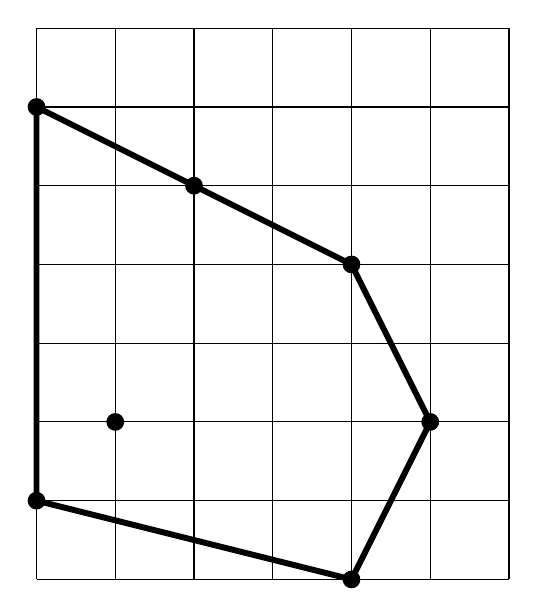
\begin{tikzpicture}
      \draw[step=1.0,black,thin] (0,0) grid (6,7);
      \filldraw (0,1) circle (3pt);
      \filldraw (5,2) circle (3pt);
      \filldraw (4,4) circle (3pt);
      \filldraw (4,0) circle (3pt);
      \filldraw (2,5) circle (3pt);
      \filldraw (1,2) circle (3pt);
      \filldraw (0,6) circle (3pt);
      \draw [line width=0.75mm] (0,1) -- (0,6) -- (2,5) -- (4,4) -- (5,2) -- (4, 0) -- (0,1);
    \end{tikzpicture}
    \caption{Newton polytope of \( f(x,y) \)} \label{fig:newton-polytope}  
  \end{subfigure}
  \begin{subfigure}[b]{0.45\linewidth}
    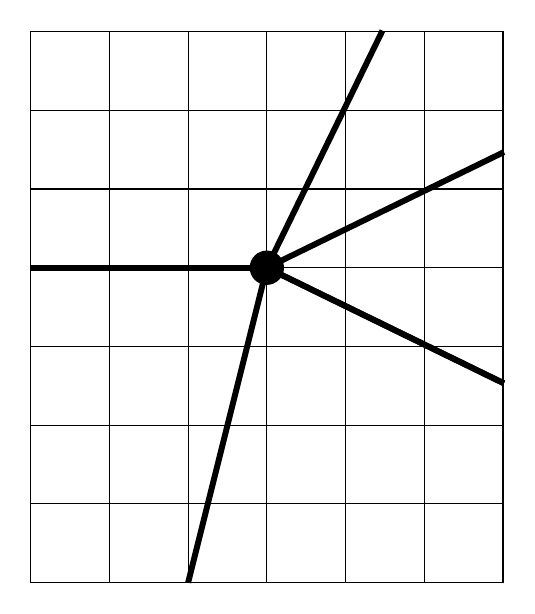
\begin{tikzpicture}
      \draw[step=1.0,black,thin] (-3,-4) grid (3,3);
      \filldraw (0,0) circle (6pt);
      \draw [line width=0.75mm] (0,0) -- (-3,0);
      \draw [line width=0.75mm] (0,0) -- (-1,-4);
      \draw [line width=0.75mm] (0,0) -- (-26:3.35);
      \draw [line width=0.75mm] (0,0) -- (-26:3.35);
      \draw [line width=0.75mm] (0,0) -- (26:3.35);
      \draw [line width=0.75mm] (0,0) -- (64:3.35);
    \end{tikzpicture}
    \caption{Normal fan of the Newton polytope} \label{fig:normal-fan-newton-polytope}  
  \end{subfigure}
\end{figure}

\begin{prop}[Useful formula]
  Let \( I \) be an ideal in \( k[\mathbf x] \). Then,
  \begin{align*}
    \mathrm{in}_{\prec_\omega} (I) = \mathrm{in}_\prec(\mathrm{in}_\omega(I)).
  \end{align*}
\end{prop}

\begin{proof}
  Reduce to the case \(  \mathrm{in}_{\prec_\omega} (f) = \mathrm{in}_\prec(\mathrm{in}_\omega(f)) \) for \( f \in I \). Then, \( \mathrm{in}_{\prec_\omega} (I)  \) and \( \mathrm{in}_\prec(\mathrm{in}_\omega(I)) \) contain the same monomials and hence are the same.
\end{proof}

If the initial ideal \( \mathrm{in}_\omega(I) \) is a monomial ideal, say it is generated by monomials \( \{f_1,\dots,f_s\} \), then we clearly found a Gröbner basis of \( \mathrm{in}_\omega(I) \) with respect to any monomial order \( \prec \). 

\begin{center}
  \emph{What if the initial ideal \( \mathrm{in}_\omega(I) \) is not a monomial ideal?\\What is the Gröbner basis?}
\end{center}

 Assume \( \mathrm{in}_\omega(I) = (g_1,\dots,g_s) \) where \( g_1,\dots,g_s \) are not necessarily monomials. We want to find a Gröbner basis, i.e. find polynomials \( f_1,\dots,f_r \) such that 
\begin{align*}
  \mathrm{in}_\prec(\mathrm{in}_\omega(I)) = \mathrm{in}_\prec(f_1,\dots,f_r).
\end{align*}

\begin{cor}[Gröbner basis of initial ideals \( \mathrm{in}_\omega \)]\label{groebner-of-inw}
  Let \( \omega \geq 0 \).
  Let \( \mathcal{G} \) be a Gröbner basis of \( I \) with respect to \( \prec_\omega \). Then \( \left\{ \mathrm{in}_\omega(g) : g \in \mathcal{G} \right\} \) is a Gröbner basis of \( \mathrm{in}_\omega(I) \) with respect to \( \prec \), i.e. 
  \begin{align*}
    \mathrm{in}_{\prec_\omega} (I) = \mathrm{in}_{\prec_\omega}(\mathcal{G}) \implies
    \mathrm{in}_\prec(\mathrm{in}_\omega (I)) = \mathrm{in}_\prec({\mathrm{in}_\omega(\mathcal{G})}).
  \end{align*}
\end{cor}

\begin{cor}[Initial ideal: weight = monomial order]
  Let \( \omega \geq 0 \). Then 
  \begin{align*}
    \mathrm{in}_{\omega}(I) \text{ is a monomial ideal} \implies \mathrm{in}_\omega(I) = \mathrm{in}_{\prec_\omega}(I).
  \end{align*}
\end{cor}


\marginnote{\small{Lec10, 06/05/23}}


\begin{mdframed}
 \begin{thm}[Representation of initial ideals]
  For all ideals \( I \subset k[\mathbf x] \)  and monomial orders \( \prec \) there exists some \( \omega \in \mathbb N^n \) such that
  \begin{align*}
    \mathrm{in}_\prec(I) = \mathrm{in}_\omega(I).
  \end{align*}
  We say \( \omega \) \textbf{represents} \( \mathrm{in}_\prec(I) \).
\end{thm}
\end{mdframed}


\begin{proof}
  Let \( \mathcal{G} = \left\{ g_1,\dots,g_s \right\} \) be a reduced Gröbner basis of \( I \) with respect to \( \prec \). We write for all \( i=1,\dots,s \):
  \begin{align*}
    g_i = c_{i0} \mathbf{x}^{\mathbf{a}_{i0}} + c_{i1} \mathbf{x}^{\mathbf a_{i1}} + \dots + c_{ij_i} \mathbf{x}^{\mathbf a_{ij_i}}, \quad \text{where } \mathbf{x}^{\mathbf{a}_{i0}} = \mathrm{in}_\prec(g_i).
  \end{align*}
  Next, we define 
  \begin{align*}
    \mathcal{C} &= \left\{ \omega \in \mathbb R_{\geq 0}^n : \mathrm{in}_\omega(g_i)= \mathbf{x}^{\mathbf{a}_{i0}}, \; \forall i=1, \dots, s \right\}  \\
    &= \left\{ 
      \omega \in \mathbb R_{\geq 0}^n :  \langle \mathbf a_{i0} - \mathbf{a}_{ij}, \omega \rangle > 0, \; \forall i=1,\dots,s; \,\forall  j = 1, \dots, j_i
     \right\}.
  \end{align*}

  \begin{itemize}
    \item Claim: any \( \omega \in \mathcal{C} \) works. Let \( \omega \in \mathcal{C} \).  We know that 
    \begin{align*}
     \mathrm{in}_\prec (I) = \mathrm{in}_\prec(g_i : i = 1, \dots, s) = (\mathbf x^{\mathbf a_{i0}} : i =1, \dots, s) \subset \mathrm{in}_\omega (I)
    \end{align*}
    because \( \mathrm{in}_\omega(g_i) = \mathbf x^{\mathbf a_{i0}} \) and \( g_i \in I \). Suppose for contradiction that \( \mathrm{in}_\prec (I) \subsetneq \mathrm{in}_\omega(I) \). Applying \( \mathrm{in}_\prec \) on both sides yields (see Corollary \ref{macaulay-cor-2}) 
    \begin{align*}
      \mathrm{in}_\prec(I) \subsetneq \mathrm{in}_{\prec_\omega}(I)
    \end{align*}
    which is not possible by Corollary \ref{macaulay-cor}.
    \item Claim: \( \mathcal{C} \neq \emptyset \). Let's rewrite \( \mathcal{C} \) as a solution set of a linear system. Define the matrix \( \mathbf A \) with rows \( (\mathbf a_{ij} - \mathbf a_{i0}) \) for all \( i,j \); that is
    \begin{align*}
      \mathbf A \coloneqq \begin{bmatrix}
        \horzbar \, (\mathbf{a}_{ij} - \mathbf{a}_{i0}) \, \horzbar \\
      \end{bmatrix}_{i=1,...,s; j = 1,...,j_i}.
    \end{align*}
    Assume \( \mathcal C \) is empty. Then \( \mathbf A \omega < \mathbf 0 \) has no solution for \( \omega \geq \mathbf 0 \).
    Let \( \mathbf b = [-1, \dots , -1] \). Then also \(  \mathbf A \omega \leq \mathbf b \) has no solution \( \omega \geq \mathbf 0 \). By \emph{Farkas Lemma}, there exists \( \mathbf c \geq 0 \) such that 
    \begin{align*}
      \mathbf{c}^T \mathbf A \geq 0 \quad \text{and} \quad \mathbf{c}^T\mathbf{b} < 0.
    \end{align*}
    Note that the vector \( \mathbf c \) has the form 
    \begin{align*}
      \mathbf  c^T = \begin{pmatrix}
        \mathbf c_{0,0} & ... &\mathbf c_{0,j_0} &\mathbf c_{1,0} & ... &\mathbf c_{1,j_1} & ... & \mathbf c_{s,0} & ... & \mathbf c_{s,j_s}
      \end{pmatrix};
    \end{align*}
    thus the elements of \( c \) are indexed by \( i,j \). So the system \( -\mathbf A^T \mathbf c \leq 0 \) yields
    \begin{align*}
      \begin{bmatrix}
        \vertbar & \vertbar & \vertbar & \vertbar \\
        \mathbf a_{10} - \mathbf a_{11} & \mathbf a_{10} - \mathbf a_{1j_1} & \dots & \mathbf a_{s0} - \mathbf a_{sj_s}\\
        \vertbar & \vertbar & \vertbar & \vertbar
      \end{bmatrix} \mathbf c = \sum_{ij} \mathbf c_{ij} \begin{bmatrix}
        \vertbar\\
        \mathbf a_{i0} - \mathbf a_{ij}\\
        \vertbar
      \end{bmatrix} \leq \mathbf 0.
    \end{align*}
    Without loss of generality we can assume that \( \mathbf c_{ij} \in \mathbb N \). Transposing again yields
    \begin{align*}
      \sum_{i,j} \mathbf c_{ij} (\mathbf a_{i0} - \mathbf a_{ij}) \leq 0.
    \end{align*}
    This translates into 
    \begin{align*}
      \prod_{i,j} (\mathbf x^{\mathbf a_{i0}})^{\mathbf c_{ij}} \preceq \prod_{i,j} (\mathbf x^{\mathbf a_{ij}})^{\mathbf c_{ij}}.
    \end{align*}
    Note that not all \( \mathbf c_{ij} \)  vanish, otherwise \( \mathbf c^T \mathbf b = 0 \). Thus, since we know that \( \mathbf x^{\mathbf a_{i0}} \succ \mathbf x^{\mathbf a_{ij}} \) from \( \mathrm{in}_\prec (g_i) = \mathbf x^{\mathbf a_{i0}}\), we get 
    \begin{align*}
      (\mathbf x^{\mathbf a_{i0}})^{\mathbf c_{ij}} \succ (\mathbf x^{\mathbf a_{ij}})^{\mathbf c_{ij}};
    \end{align*}
    thus 
    \begin{align*}
      \prod_{i,j} (\mathbf x^{\mathbf a_{i0}})^{\mathbf c_{ij}} \succ \prod_{i,j} (\mathbf x^{\mathbf a_{ij}})^{\mathbf c_{ij}}
    \end{align*}
    This is a contradiction. So \( \mathcal{C} \neq \emptyset \).
  \end{itemize}
\end{proof}

Fix an ideal \( I \subset k[x_1,...,x_n] \). We define an \textbf{equivalence relation} on \( \omega \in \mathbb R^n \) by \( \omega \sim \omega' \) if \( \mathrm{in}_{\omega}(I) = \mathrm{in}_{\omega'}(I) \). The \textbf{equivalence class} of \( \omega \) is denoted 
\begin{align*}
  C_I[\omega] = \left\{ \omega \in \mathbb R^n : \mathrm{in}_{\omega}(I) = \mathrm{in}_{\omega '}(I) \right\}.
\end{align*}
We will see that \( C_I[\omega] \) is in fact a polyhedral cone.

\begin{defi}[Equivalent weight vector]
  We say two weight vectors \( \omega, \omega' \in \mathbb R^n \) are \textbf{equivalent}\index{weight vector!equivalent} (with respect to \( I \)) if \( \omega \sim \omega' \).
\end{defi}

\begin{defi}[Gröbner region]
  The \textbf{Gröbner region} of an ideal \( I \) is defined as 
  \begin{align*}
    \mathrm{GR}(I) = \left\{ \omega \in \mathbb R^n : \omega \sim \omega' \text{ for some \( \omega' \in \mathbb R^n_{\geq 0} \)} \right\}.
  \end{align*}
\end{defi}

\begin{remark}
  The Gröbner region always contains \( \mathbb R^n_{\geq 0} \).
\end{remark}

\begin{remark}[Gröbner region = support of Gröbner fan]
  We will later see that closure of the Gröbner region \( \overline{\mathrm{GR}(I)} \) is the support of the Gröbner fan of \( I \).
\end{remark}

\begin{eg}
  Here is the Gröbner region of \( I \). Note that any \( \omega \) outside the Gröbner region cannot be monomial orders. For instance, if \( y \) were the leading term of \( I \), then \( y^6 \prec y \) but this is not possible because \( y \) divides \( y^6 \).
  \begin{figure}[H]
    \centering
      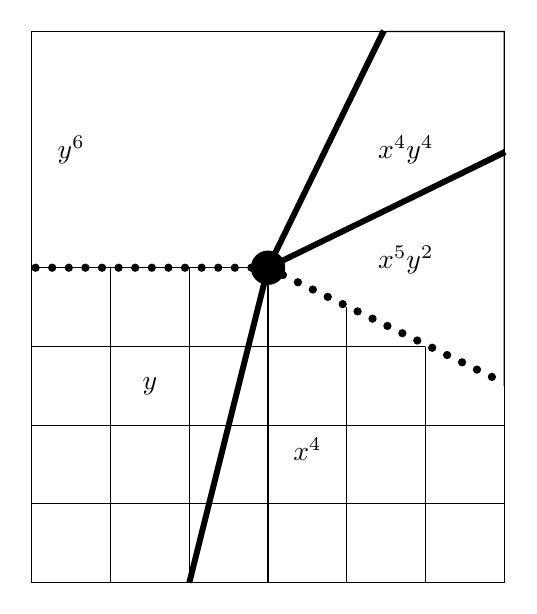
\begin{tikzpicture}
        \draw[step=1.0,black,thin] (-3,-4) grid (3,3);
        \draw[fill=white] (0,0) -- (-3,0) -- (-3,3) -- (1.5, 3);
        \draw[fill=white] (0,0) -- (1.5,3) -- (3,3) -- (3, 1.3);
        \draw[fill=white] (0,0) -- (3,1.5) -- (3,-1.5);
        \filldraw (0,0) circle (6pt);
        \draw [line width=3pt, line cap=round, dash pattern=on 0pt off 2\pgflinewidth] (0,0) -- (-3,0);
        \draw [line width=0.75mm] (0,0) -- (-1,-4);
        \draw [line width=3pt, line cap=round, dash pattern=on 0pt off 2\pgflinewidth] (0,0) -- (-26:3.35);
        \draw [line width=0.75mm] (0,0) -- (26:3.35);
        \draw [line width=0.75mm] (0,0) -- (64:3.35);
        \draw (-1.5,-1.5) node {\( y \)};
        \draw (-2.5,1.5) node {\( y^6 \)};
        \draw (1.75,1.5) node {\( x^4 y^4 \)};
        \draw (1.75,0.1) node {\( x^5 y^2 \)};
        \draw (0.5,-2.3) node {\( x^4 \)};
      \end{tikzpicture}
      \caption{The white area is the Gröbner region of \( I \).}
  \end{figure}
\end{eg}





\subsection{Gröbner Fan}
\marginnote{\small{Lec11, 06/06/23}}

Our goal in this section is to prove the existence of the Gröbner fan. 

Recall that we defined two weight vectors to be equivalent with respect to \( I \) if \( \mathrm{in}_\omega(I) = \mathrm{in}_{\omega'}(I) \). It turns out that if \( \omega \in \mathbb R^n_{\geq 0} \) it suffices to check that they are equivalent with respect to the reduced Gröbner basis of \( I \) (for some monomial order \( \prec_\omega \)). 

\begin{remark}\label{facenewf}
  Observe that we have the following fact 
  \begin{align*}
    \mathrm{face}_\omega(\mathrm{New}(f)) = \mathrm{New}(\mathrm{in}_\omega(f)).
  \end{align*}
  Proof. Take a vertex \( \alpha_j \in  \mathrm{face}_\omega(\mathrm{New}(f)) \). Then it is easy to see that \( \alpha_j \in   \mathrm{New}(\mathrm{in}_\omega(f))\). The converse direction is similar.
\end{remark}

\begin{prop}
  \( \mathrm{New}(f \cdot g) = \mathrm{New}(f) + \mathrm{New}(g) \).
\end{prop}

\begin{prop}\label{groebner-fan-lemma}
  Fix an ideal \( I \subset k[x_1,...,x_n] \) and \( \omega \in \mathbb R^n_{\geq 0} \). Let \( \mathcal{G} = \left\{ g_1,...,g_s \right\} \) be the reduced Gröbner basis of \( I \) with respect to \( \prec_\omega \) for some monomial order \( \prec \). Then, we have 
  \begin{align*}
    C_I[\omega] = \left\{ \omega' \in \mathbb R^n : \mathrm{in}_{\omega'}(g_i) = \mathrm{in}_\omega(g_i) \; \forall i = 1, \dots , s \right\}.
  \end{align*}
\end{prop}

\begin{proof}\(  \)

  \begin{itemize}
    \item \( \supset \): Let \( \omega' \in \left\{ \omega' \in \mathbb R^n : \mathrm{in}_{\omega'}(g_i) = \mathrm{in}_\omega(g_i) \; \forall i = 1,..., s \right\} \). Then 
    \begin{align*}
      \mathrm{in}_{\omega'}(I) \supset (\left\{  \mathrm{in}_{\omega'}(g_i) \; \forall i = 1,..., s \right\}) = (\left\{  \mathrm{in}_{\omega}(g_i) : \forall i = 1,..., s \right\} ) = \mathrm{in}_\omega(I)
    \end{align*}
    where the last equality follows from Corollary \ref{groebner-of-inw}. Assume for contradiction that the inclusion were strict, i.e. \( \mathrm{in}_{\omega '}(I) \supsetneq \mathrm{in}_{\omega}(I) \). By Corollary \ref{macaulay-cor-2}, we have \( \mathrm{in}_{\prec_{\omega'}}(I) \supsetneq \mathrm{in}_{\prec_\omega}(I)\). This contradicts Corollary \ref{macaulay-cor}. Hence, \( \mathrm{in}_{\omega '}(I) = \mathrm{in}_{\omega}(I)  \), and therefore \( \omega' \in C_I[w] \).

    \item \( \subset \): Let \( \omega' \in C_I[\omega] \). By Corollary \ref{groebner-of-inw} we have \( \{ \mathrm{in}_{\omega}(g_i) : \forall i = 1,..., s \} \) is a Gröbner basis of \( \mathrm{in}_\omega(I) = \mathrm{in}_{\omega ' }(I) \) with respect to \( \prec \). We also have \( \mathrm{in}_{\omega'}(g_i) \in \mathrm{in}_{\omega'}(I) \), and we just saw that \( \mathrm{in}_{\omega'}(I) \) has Gröbner basis \( \{ \mathrm{in}_{\omega}(g_i) : \forall i = 1,..., s \} \). So,   
    \begin{align*}
      \overline{\mathrm{in}_{\omega '}(g_i)}^{\mathrm{in}_\omega(\mathcal{G})} = 0.
    \end{align*}
    Let \( m = \mathrm{in}_{\prec_\omega}(g_i) \). It is the only monomial of \( g_i \) divisible by any of \( \mathrm{in}_\prec(\mathrm{in}_\omega(g_j)), j = 1, ... , s \) since \( \mathcal{G} \) is reduced. Assume that \( m \) does not appear in \( \mathrm{in}_{\omega'}(g_i) \), so there is some other monomial of \( g_i \) whose residue vanishes with respect to \( \mathrm{in}_\omega(G) \). This means that this monomial is divisible by \( \mathrm{in}_\prec(\mathrm{in}_\omega (g_j)) \) which is not possible. Thus, \( m \) appears in \( \mathrm{in}_{\omega'}(g_i) \).

    Write \( \mathrm{in}_{\omega}(g_i) = m + h\in \mathrm{in}_\omega( I ) \) and  \( \mathrm{in}_{\omega'}(g_i) = m + h' \in \mathrm{in}_\omega( I ) \) for some \( h, h' \notin \mathrm{in}_{\prec_\omega}(I) \) (if \( h, h' \in  \mathrm{in}_{\prec_\omega}(I) \), then \( \mathcal{G} \) would not be reduced). Subtracting yields \( h - h ' \in \mathrm{in}_\omega( I )\). Assume \( h - h' \neq 0 \). Then \( \mathrm{in}_\prec(h - h') \in \mathrm{in}_{\prec_\omega}(I) \). This is a contradiction because no term of \( h, h' \) is divisible by \( \mathrm{in}_{\prec_\omega}(I) \).

    We obtain \( \mathrm{in}_\omega(g_i) = m = \mathrm{in}_{\omega'}(g_i) \).
  \end{itemize}
\end{proof}

\begin{cor}\label{ci-geometric}
  Let \( \mathcal{N}_P(F) \) denote the normal cone of a polytope \( P \) with face \( F \subset P \). The previous proposition shows that 
  \begin{align*}
    C_I[\omega] = \mathrm{\mathcal{N}}_{\mathrm{New}(\prod g)}(\mathrm{face}_\omega(\mathrm{New}(\prod g))).
  \end{align*}

\begin{proof}
  Take \( \omega' \in \mathrm{\mathcal{N}}(\mathrm{face}_\omega(\mathrm{New}(\prod g))) \). By definition of the normal cone \( \mathcal{N} \), we have \( \mathrm{face}_{\omega'}(\mathrm{New}(\prod g)) = \mathrm{face}_\omega(\mathrm{New}(\prod g)) \). Thus, by Remark \ref{facenewf} we get 
  \begin{align*}
    \mathrm{New}( \mathrm{in}_{\omega'}(\prod g)) =    \mathrm{New}( \mathrm{in}_\omega(\prod g)). 
  \end{align*}
  Hence, 
  \begin{align*}
    \sum \mathrm{New}(\mathrm{in}_{\omega'}(g)) = \mathrm{New}(\prod \mathrm{in}_{\omega'}( g)) =    \mathrm{New}(\prod  \mathrm{in}_\omega( g)) =  \sum \mathrm{New}(\mathrm{in}_{\omega}(g)). 
  \end{align*}
  Hence, \( \mathrm{New}(\mathrm{in}_{\omega'}(g)) = \mathrm{New} (\mathrm{in}_{\omega}(g)) \) for all \( g \in \mathcal{G} \). Therefore, the vertices of the newton polytopes coincide which means that \( \mathrm{in}_{\omega'}(g) \) and \( \mathrm{in}_{\omega}(g) \) coincide. Thus, \( \omega' \in C_I[\omega] \). The reverse direction is similar.
\end{proof}
\end{cor}

\begin{mdframed}
\begin{cor}[Polyhedral cone]
  Let \( I \) be an ideal in \( k[x_1, \dots, x_n] \) and \( \omega \in \mathbb R^n \). If \( \omega \geq 0 \), then \( C_I[\omega] \) is a relatively open polyhedral cone in \( \mathbb R^n \).
\end{cor}
\end{mdframed}

\begin{proof}
  By the previous proposition we have 
  \begin{align*}
    C_I[\omega] = \left\{ \omega' \in \mathbb R^n : \mathrm{in}_{\omega'}(g_i) = \mathrm{in}_\omega(g_i) \; \forall i = 1, \dots , s \right\}.
  \end{align*}
  Write \( g_i = \sum \lambda_{\alpha}  x^{\alpha} + \sum \lambda_{\beta} x^{\beta} \) such that \( \mathrm{in}_{\omega}(g_i) = \sum \lambda_\alpha x^{\alpha} \). Then \( \mathrm{in}_{\omega'}(g_i) = \mathrm{in}_\omega(g_i) \) means that 
  \begin{align*}
    \alpha \cdot \omega' = \alpha \cdot \omega' \quad \text{ and } \quad    \alpha \cdot \omega' > \beta \cdot \omega'\qquad  \forall \alpha, \beta.
  \end{align*}
  Hence, 
  \begin{align*}
    C_I[\omega] = \left\{ \omega' \in \mathbb R^n :    \underbrace{ \alpha_{} \cdot \omega' = \alpha_{} \cdot \omega'}_{\text{defines linear subspace}},  \underbrace{ \alpha \cdot \omega' > \beta \cdot \omega'}_{\text{defines cone}}  \; \forall i = 1, \dots , s, \forall \alpha, \beta \right\}.
  \end{align*}
\end{proof}

\begin{cor}[Gröbner cone]
  Let \( I \) be an ideal in \( k[x_1, \dots, x_n] \) and \( \omega \in \mathbb R^n \). If \( \omega \geq 0 \), then 
  \begin{align*}
    \overline{C_I[\omega]} = \left\{ \omega ' \in \mathbb R^n : \mathrm{in}_\omega(\mathrm{in}_{\omega'}(g_i)) = \mathrm{in}_\omega(g_i) \; \forall i = 1, \dots, s \right\}.
  \end{align*}
  This closed polyhedral cone is called \textbf{Gröbner cone}\index{Gröbner cone}.
\end{cor}

\begin{proof}
  Use 
  \begin{align*}
    \overline{C_I[\omega]} = \left\{ \omega' \in \mathbb R^n :    \alpha_{} \cdot \omega' = \alpha_{} \cdot \omega',   \alpha \cdot \omega' \geq \beta \cdot \omega'  \; \forall i = 1, \dots , s, \forall \alpha, \beta \right\}.
  \end{align*}
  (Here is a dirty proof: If \( \alpha_{}  \omega' = \alpha_{}  \omega' \) and \( \alpha \omega' \geq \beta \omega' \), then after taking \( \mathrm{in}_\omega(\bullet) \) only the monomials with \( \alpha \omega ' > \beta \omega ' \) survive. This proves \( \subset \).

  For \( \supset \), take \( \omega' \) from the right-hand side. Hence, \( \mathrm{in}_{\omega'}(g_i) \) contains monomials \( x^\alpha \). It may contain other monomials \( x^\gamma \). Thus, \( w' \alpha = w' \gamma \) and \( w' \alpha >  w' \beta' \). Hence, \( \alpha w ' = \alpha w' \) and \( \alpha w' \geq \beta w' \) for \( \beta\in \left\{ \gamma, \beta' \right\} \).)
  
\end{proof}

\begin{eg}[\( \omega \geq 0 \) is necessary]
  The assumption \( \omega \geq 0 \) is necessary. Let \( I = (x-1, y-1) \subset \mathbb R[x,y] \).  For \( \omega_1 = (3, -1) \) and \( \omega_2 = (-1, 3) \) we have \( \mathrm{in}_{\omega_1}(I) = \mathrm{in}_{\omega_2}(I) = (-1) = (1) \). However, \( \omega = \frac{\omega_1 + \omega_2}{2} = (2,2) \) and hence \( \mathrm{in}_{\omega}(I) = (x,y) \). Thus, \( \omega \notin C_I[\omega_1] = C_I[\omega_2] \) which shows that \( C_I[\omega_1] \) is not a cone.


\begin{figure}[H]
  \centering
  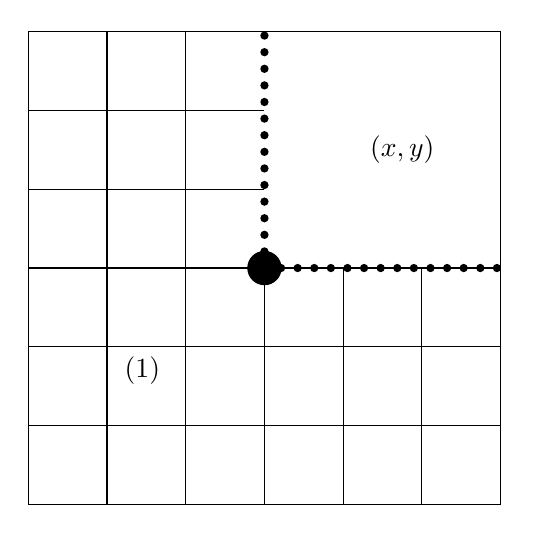
\begin{tikzpicture}
    \draw[step=1.0,black,thin] (-3,-3) grid (3,3);
    \draw[fill=white] (0,0) -- (3,0) -- (3,3) -- (0, 3);
    \draw [line width=3pt, line cap=round, dash pattern=on 0pt off 2\pgflinewidth] (0,0) -- (3,0);
    \draw [line width=3pt, line cap=round, dash pattern=on 0pt off 2\pgflinewidth] (0,0) -- (0,3);
    \draw (1.75,1.5) node {\((x,y) \)};
    \draw (-1.55,-1.3) node {\((1) \)};
    \filldraw (0,0) circle (6pt);
  \end{tikzpicture}
\end{figure}
\end{eg}

\marginnote{\small{Lec12, 06/12/23}}
\begin{defi}[Gröbner fan]\index{Gröbner fan}
  Let \( I \subset k[x_1, \dots, x_n] \) be an ideal. We define 
  \begin{align*}
    \mathrm{GFan}(I) = \left\{ \overline{C_I[\omega]} \; | \; \omega \in \mathbb R^n_{\geq 0} \right\}.
  \end{align*}
\end{defi}

\begin{remark}
  The closure \( \overline{\bullet} \) is to be understood as the relative closure in \( \mathrm{GR}(I) \).
\end{remark}


\begin{lemma}
  Let \( I \subset k[x_1, \dots, x_n] \) be an ideal and \( \omega \in \mathbb R^n_{\geq 0} \). Then, 
  \begin{align*}
    \omega' \in \overline{C_I[\omega]} \implies \text{ \( \overline{C_I[\omega']} \) is a face of \( \overline{C_I[\omega]} \)}.
  \end{align*}
\end{lemma}

\begin{proof}
  Fix any monomial order \( \prec \) and let \( \mathcal{G} \) be the reduced Gröbner basis of \( I \) with respect to \( \prec_\omega \). Let \( \omega' \in \overline{C_I[\omega]} \). 

  \begin{itemize}
    \item  We have \(  \mathrm{in}_\omega(\mathrm{in}_{\omega'}(g)) = \mathrm{in}_\omega(g) \) for all \( g \in \mathcal{G} \).
    \item Define \( J = (\mathrm{in}_{\omega'}(g) : g \in \mathcal{G} \subset I) \subset \mathrm{in}_{\omega'}(I) \).
    \item By Corollary \ref{groebner-of-inw} we have \( \mathrm{in}_\omega(I) = (\mathrm{in}_\omega(g) : g \in \mathcal{G}) \subset \mathrm{in}_{\omega}(J) \) (use the first bullet point)
    \item Applying \( \mathrm{in}_{\prec} (\bullet)\) yields \( \mathrm{in}_{\prec_\omega}(I) \subset \mathrm{in}_{\prec_\omega}(J) \subset \mathrm{in}_{\prec_\omega}(\mathrm{in}_{\omega'}(I)) = \mathrm{in}_{(\prec_\omega)_{\omega'}}(I) \)
  \end{itemize}

  By Macaulay's Corollary \ref{macaulay-cor} all inclusions are equality, that is \(  \mathrm{in}_{\prec_\omega}(I ) =  \mathrm{in}_{(\prec_\omega)_{\omega'}}(I)  \).
  Since \( \mathcal{G} \)  is a Gröbner basis of \( I \) we have \( \mathrm{in}_{\prec_\omega}(\mathcal{G}) = \mathrm{in}_{\prec_\omega}(I )  \). Note that \( \mathrm{in}_{\prec_\omega}(\mathcal{G}) = \mathrm{in}_{\prec}(\mathrm{in}_{\omega}(\mathrm{in}_{\omega'}(\mathcal{G}))) = \mathrm{in}_{(\prec_{\omega})_{\omega'}}(\mathcal{G}) \). Hence,
  \begin{align*}
    \mathrm{in}_{(\prec_{\omega})_{\omega'}}(\mathcal{G}) = \mathrm{in}_{\prec_\omega}(\mathcal{G}) = \mathrm{in}_{\prec_\omega}(I ) =  \mathrm{in}_{(\prec_\omega)_{\omega'}}(I) 
  \end{align*}
  which shows that \( \mathcal{G} \) is a reduced Gröbner basis of \( I \) with respect to \( (\prec_\omega)_{\omega'} \). Applying Proposition \ref{groebner-fan-lemma} yields 
  \begin{align*}
    \overline{C_I[\omega']} = \left\{ \omega '' \in \mathbb R^n : \mathrm{in}_{\omega'}(\mathrm{in}_{\omega''}(g)) = \mathrm{in}_{\omega'}(g) \; \forall g \in \mathcal{G} \right\}.
  \end{align*}
  Note that any \( \omega'' \in  \overline{C_I[\omega']} \) satisfies \(  \mathrm{in}_\omega(\mathrm{in}_{\omega''}(g)) = \mathrm{in}_\omega(g) \) for all \( g \in \mathcal{G} \). Hence, \(   \overline{C_I[\omega']} \subset   \overline{C_I[\omega]} \). Moreover, transforming \(  \mathrm{in}_{\omega'}(\mathrm{in}_{\omega''}(g)) = \mathrm{in}_{\omega'}(g)  \) into a set of linear equalities and inequalities \( \omega'' \alpha = \omega '' \alpha \) and \( \omega'' \alpha > \omega'' \beta \) reveals that the set of \( \beta \)'s is a subset of the set of \( \beta \)'s of \( \overline{C_I[\omega]} \) (the missing inequality becomes an equality in \( \overline{C_I[\omega']} \)). Hence, \(  \overline{C_I[\omega']} \) is a face of \(  \overline{C_I[\omega]} \).
\end{proof}

\begin{mdframed}
  \begin{thm}[Gröbner fan is a polyhedral fan]
    Let \( I \subset k[x_1, \dots, x_n] \) be an ideal. Then \( \mathrm{GFan}(I) \) is a polyhedral fan.
  \end{thm}
\end{mdframed}

\begin{proof}\(  \)
  \begin{itemize}
    \item All faces are in the fan: let \( F \) be a face of \( \overline{C_I[\omega]} \). Take \( \omega' \in \mathbb R^n_{\geq 0} \) in the relative interior and by the previous lemma we have \( \overline{C_I[\omega']} \) is a face. Note that \( F \) is the only possible face of \( \overline{C_I[\omega]} \) that can contain a relative interior \( \omega' \). Hence, \( F = \overline{C_I[\omega']} \).
    \item Intersection of two cones in \( \mathrm{GRFan} \) is a common face: let \( P = \overline{C_I[\omega]} \cap \overline{C_I[\omega']} \). Take any \( \omega'' \in P \). Then \( \overline{C_I[\omega'']} \) is a common face of \( \overline{C_I[\omega]} \) and \( \overline{C_I[\omega']} \). Hence, \( P = \bigcup_{\omega'' \in P} \overline{C_I[\omega'']} \). Since \( P \) is convex, the union is a singleton. So \( P \) is a common face.
  \end{itemize}
\end{proof}

\begin{eg}
  The Gröbner fan of \( I = (f)\) where \(     f(x,y) = x^5y^2 + x^4y^4 + x^4 + x^2y^5 + xy^2 + y^6 + y
 \) is 
  \begin{figure}[H]
    \centering
      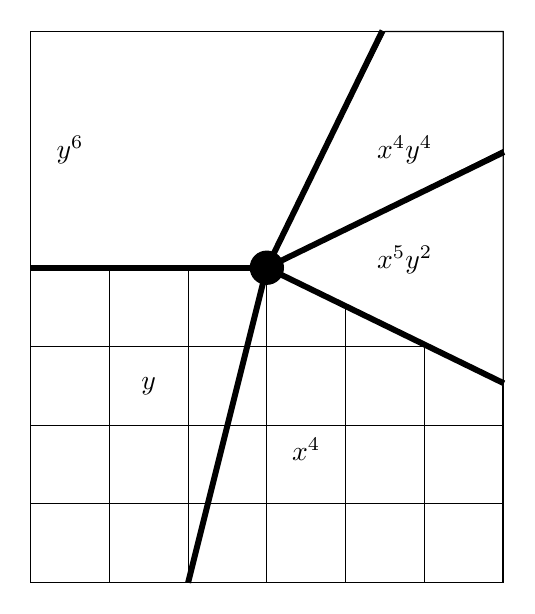
\begin{tikzpicture}
        \draw[step=1.0,black,thin] (-3,-4) grid (3,3);
        \draw[fill=white] (0,0) -- (-3,0) -- (-3,3) -- (1.5, 3);
        \draw[fill=white] (0,0) -- (1.5,3) -- (3,3) -- (3, 1.3);
        \draw[fill=white] (0,0) -- (3,1.5) -- (3,-1.5);
        \filldraw (0,0) circle (6pt);
        \draw [line width=0.75mm] (0,0) -- (-3,0);
        \draw [line width=0.75mm] (0,0) -- (-1,-4);
        \draw [line width=0.75mm] (0,0) -- (-26:3.35);
        \draw [line width=0.75mm] (0,0) -- (26:3.35);
        \draw [line width=0.75mm] (0,0) -- (64:3.35);
        \draw (-1.5,-1.5) node {\( y \)};
        \draw (-2.5,1.5) node {\( y^6 \)};
        \draw (1.75,1.5) node {\( x^4 y^4 \)};
        \draw (1.75,0.1) node {\( x^5 y^2 \)};
        \draw (0.5,-2.3) node {\( x^4 \)};
      \end{tikzpicture}
      \caption{The Gröbner fan \( I \).}
  \end{figure}
\end{eg}

\begin{eg}
  Let \( f \) be homogeneous.
  To draw the Gröbner fan of a principal ideal \( I = (f) \) do the following: Draw the Newton polytope of \( f \) and then draw the normal fan of this Newton polytope. The Gröbner fan consists of cones intersecting the non-negative orthant.
\end{eg}


\begin{eg}
  Let \( I = (x-1, y-1) \). An universal Gröbner basis is given by \( \mathcal{G} = \left\{ x-1, y-1 \right\} \) (check by computing the \( S \)-polynomial). There is a one-to-one correspondence between \( \mathrm{in}_{\omega}(I) \) where weights \( \omega \geq 0 \) represent a monomial ideal and \( \mathrm{in}_{\prec}(I) \). Thus, there is only one maximal cone in \( \mathrm{GFan} \) since \( \mathrm{in}_{\prec}(I) = \mathrm{in}_\prec(\mathcal{G}) = (x,y) \) for all monomial orders \( \prec \) (in other words, there exists exactly one initial ideal of \( I \)). In order to represent \( (x,y) \), \( \omega \) may only take non-negative values.
  \begin{figure}[H]
    \centering
    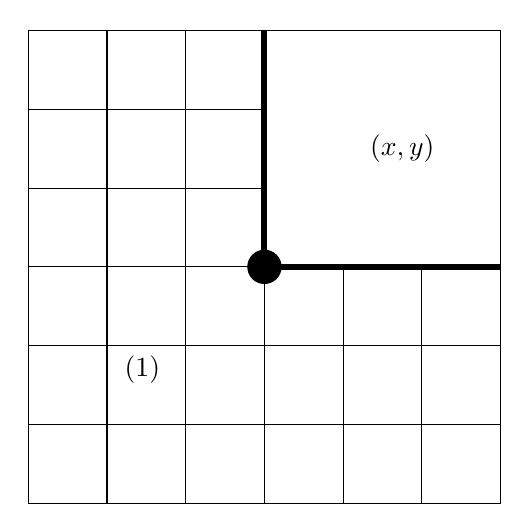
\begin{tikzpicture}
      \draw[step=1.0,black,thin] (-3,-3) grid (3,3);
      \draw[fill=white] (0,0) -- (3,0) -- (3,3) -- (0, 3);
      \draw [line width=0.75mm] (0,0) -- (3,0);
      \draw [line width=0.75mm] (0,0) -- (0,3);
      \draw (1.75,1.5) node {\((x,y) \)};
      \draw (-1.55,-1.3) node {\((1) \)};
      \filldraw (0,0) circle (6pt);
    \end{tikzpicture}
  \end{figure}
\end{eg}

\begin{remark}[How to draw the Gröbner fan by hand]
  Assume \( I = (f_1, \dots, f_s) \). Compute a universal Gröbner basis \( \mathcal{G} \). Then, compute all the possible initial ideals \( \mathrm{in}_{\prec}(\mathcal{G}) \); for example, say we have \( \mathrm{in}_{\prec}(\mathcal{G}) = (x^{\alpha_1}, ... , x^{\alpha_s}) \). Write inequalities \( \omega \alpha_i > \omega \beta_i \) where \( f_i = \lambda_{\alpha_i} x^{\alpha_i} + \sum_{\beta_i} \lambda_{\beta_i} x^{\beta_i} \). Draw the cones \( \omega \in \mathbb R^n \) defined by \(  \omega \alpha_i > \omega \beta_i  \).

  Repeat this process for every possible initial ideal \( \mathrm{in}_\prec(\mathcal{G}) \) varying over \( \prec \).
\end{remark}


\begin{eg}
  Let \( I = ( y^2 + xy + 1, x^2) \subset k[x,y] \).

  \begin{itemize}
    \item Take a monomial order defined by \( \omega = (1,2) \). Then, \( \mathrm{in}_\omega(y^2 + xy + 1) = y^2 \) and \( \mathrm{in}_\omega(x^2) = x^2 \). We see that \( \mathcal{G} = \left\{ y^2 + xy + 1, x^2 \right\} \) is a reduced Gröbner basis. Hence, \( \mathrm{in}_\omega(I) = (x^2, y^2) \). Then 
    \begin{align*}
      C_I[(1,2)] &= \left\{ (\omega_1, 
      \omega_2) \in \mathbb R^2 : 2\omega_2 > \omega_1 + \omega_2, 2\omega_2 > 0 \right\} \\ &= \left\{ (\omega_1, 
      \omega_2) \in \mathbb R^2 : \omega_2 > \omega_1 , \omega_2 > 0 \right\}.
    \end{align*}

    \item Take grlex as a monomial order. We want to find \( \omega \in \mathbb R^n_{\geq 0} \) representing grlex. A Gröbner basis is given by \( \mathcal{G} = \left\{ y^2 + xy + 1, x^2, y^3 - x + y \right\} \).

    \item Take lex as a monomial order.
  \end{itemize}

  \begin{figure}[H]
    \centering
      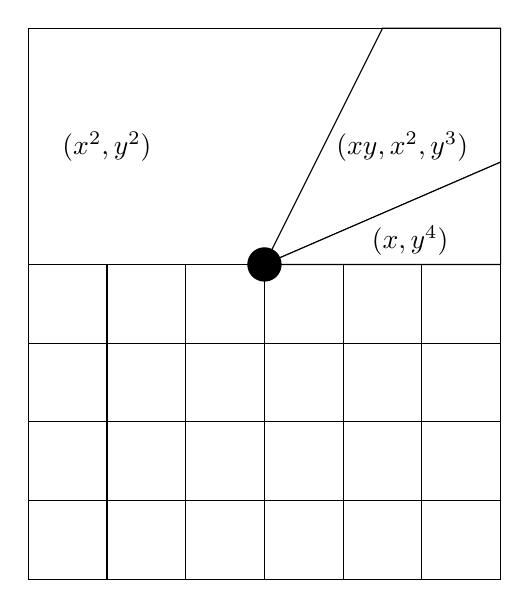
\begin{tikzpicture}
        \draw[step=1.0,black,thin] (-3,-4) grid (3,3);
        \draw[fill=white] (0,0) -- (-3,0) -- (-3,3) -- (2.5, 3);
        \draw[fill=white] (0,0) -- (1.5,3) -- (3,3) -- (3, 1.3) -- (0,0);
        \draw[fill=white] (0,0) -- (3,0) -- (3,1.3)-- (0,0);
        \filldraw (0,0) circle (6pt);
        \draw (-2.0,1.5) node {\( (x^2,y^2) \)};
        \draw (1.75,1.5) node {\( (xy,x^2,y^3) \)};
        \draw (1.85,0.3) node {\( (x,y^4) \)};
      \end{tikzpicture}
      \caption{The Gröbner fan \( I \).}
  \end{figure}
\end{eg}

\subsection{Homogeneity}
\marginnote{\small{Lec13, 06/13/23}}

\begin{defi}\index{\( \omega \)-homogeneous}
  Let \( \omega \in \mathbb R^n \). 
  \begin{itemize}
    \item   A polynomial \( f \in k[ x_1, \dots, x_n] \) is \textbf{\( \omega \)-homogeneous} if \( \mathrm{in}_\omega(f) = f \). 

    \item An ideal is \( \omega \)-homogeneous if it has an \textbf{\( \omega \)-homogeneous} generating set.
  \end{itemize}
  
\end{defi}

\begin{defi}
  An ideal is \textbf{homogeneous} if it is \( \omega \)-homogeneous for some positive \( \omega \in \mathbb R^n_{> 0} \).
\end{defi}

\begin{defi}\index{\( \omega \)-degree}
  Let \( f = \sum \lambda_\alpha x^\alpha \) be \( \omega \)-homogeneous. Its \textbf{\( \omega \)-degree} is \( \omega \cdot \alpha \).
\end{defi}

\begin{eg}[Total degree]\index{total degree}
The total degree is given by the \( \mathbf 1 = (1, \dots, 1) \)-grading.
\end{eg}

\begin{eg}\(  \)
  \begin{itemize}
    \item   Let \( f = x^3 + y^2z + z^3 \). \( f \) is \( (1,1,1) \)-homogeneous with \( \omega \)-degree \( 3 \).
    \item Let \( f = x^2 - y \). \( f \) is \( (1,2) \)-homogeneous with \( \omega \)-degree \( 2 \).
  \end{itemize}
\end{eg}

\begin{eg}
  Let \( I = (x-y, x^2 - y + y^2  + y) \). The ideal \( I \) is homogeneous because it is generated by \( (x-y, x^2 + y^2) \) and the generators are \( (1,1) \)-homogeneous polynomials.
\end{eg}

\begin{eg}
  \( I = (x-1) \) is not homogeneous because \( \mathrm{in}_\omega(x-1) = x \) for all \( \omega > 0 \).
\end{eg}

\begin{remark}
  Let \( I \) be an ideal and \( \omega \in \mathbb R^n \). Then \( \mathrm{in}_\omega(I) \) is \( \omega \)-homogeneous because \( \mathrm{in}_\omega(I) = \left\{  \mathrm{in}_\omega(f) : f \in I \right\} \) and \( \mathrm{in}_\omega(\mathrm{in}_\omega(f)) = \mathrm{in}_\omega(f) \).
\end{remark}


\begin{remark}[Unique decomposition into \( \omega \)-homogeneous parts]
  Fix \( \omega \in \mathbb R^n \). Let \( f \) be not \( \omega \)-homogeneous. Then \( f \) can be \emph{uniquely} decomposed into \( \omega \)-homogeneous parts: 
  \begin{align*}
    f = f_1 + \dots + f_j \quad \text{where \( f_j \) is \( \omega \)-homogeneous of different \( \omega \)-degree}.
  \end{align*}
\end{remark}

\begin{remark}
  Two observations:
  \begin{itemize}
    \item if \( f \) is \( \omega \)-homogeneous, then \( x^\alpha \cdot f \) is \( \omega \)-homogeneous
    \item if \( f,g \) are \( \omega \)-homogeneous of same \( \omega \)-degree, then \( f + g \) is \( \omega \)-homogeneous.
  \end{itemize}
\end{remark}

\begin{mdframed}
\begin{prop}[Characterization of \( \omega \)-homogeneous ideals]
  Let \( I \subset k[x_1, \dots, x_n] \) be an ideal and \( \omega \in \mathbb R^n_{>0} \). The following are equivalent 
  \begin{enumerate}
    \item \( I \) is \( \omega \)-homogeneous
    \item \( f \in I \) with \(f = \sum f_j \; \omega \)-homogeneous decomposition \( \implies f_j \in I \; \forall i\) 
    \item \( \mathrm{in}_\omega (I) = I \)
    \item the reduced Gröbner basis (with respect to any order \( \prec \)) of \( I \) consists of \( \omega \)-homogeneous polynomials
  \end{enumerate}
\end{prop}
\end{mdframed}

\begin{proof}\(  \)
  \begin{itemize}
    \item \(4. \implies \) (1) is clear
    \item  \(3. \implies \) (1): take \( \mathrm{in}_\omega(I) \) as a generating set of \( I \). We saw that \( \mathrm{in}_\omega(I) \) is \( \omega \)-homogeneous.
    \item \(2. \implies \) (1): By Hilbert's Basis theorem, \( I = (g_1, \dots, g_s) \). Write each \( g_i \) as a unique decomposition into \( \omega \)-homogeneous parts: \( g_i = \sum g_{ij} \). Then \( I \) is generated by \( \omega \)-homogeneous \( g_{ij} \).
    \item \( 1. \implies 4. \): By assumption \( I = (H) \)  for some (infinite) generating set \( H \) that is \( \omega \)-homogeneous. On the other hand, by Hilbert's basis theorem, there exists finite \( F \) that generates \( I \). Hence, there exists finite \( H' \subset H \) such that \( H' \) generates \( I \).
    
    Now that \( H' \) is finite, we apply Buchberger's algorithm to construct a Gröbner basis. We see that Buchberger's algorithm only appends \( \omega \)-homogeneous polynomials.

    \item \( 4. \implies 3. \) We have \( I = (G) = (\mathrm{in}_\omega(G)) \subset \mathrm{in}_\omega(I) \). This inclusion cannot be strict, if it were strict, we apply \( \mathrm{in}_\prec(\bullet) \) on both sides and by Macaulay's Corollary we obtain a contradiction.

    \item \( 4. \implies 2. \) Let \( G = \left\{ g_1, \dots, g_s \right\} \) be a reduced Gröbner basis that is \( \omega \)-homogeneous. Let \( f \in I \). Write \( f = \sum h_i g_i \) and expand \( h_i = \sum \lambda_{\alpha_i} x^{\alpha_i} \) to: \( f = \sum_{i, \alpha_i} \lambda_{\alpha_i} x^{\alpha_i} g_i \). Note that \( \lambda_{\alpha_i} x^{\alpha_i} g_i \) is \( \omega \)-homogeneous. So any \( \omega \)-homogeneous part of \( f \) is of the form \( f_j = \sum_{i, \alpha_i}  \lambda_{\alpha_i} x^{\alpha_i} g_i  \in I\) because \( g_i \in I \).
  \end{itemize}
\end{proof}

\begin{lemma}
  Let \( I \) be a \( d \)-homogeneous ideal for some \( d > 0 \). Let \( \omega \in \mathbb R^n \). Then \( \mathrm{in}_\omega(I) = \mathrm{in}_{\omega + \lambda d}(I) \) for every \( \lambda \in \mathbb R \).
\end{lemma}

\begin{proof}
  If \( f \) is \( d \)-homogeneous, then \( \mathrm{in}_\omega(f) = \mathrm{in}_{\omega + \lambda d}(f)  \) for all \( \lambda \in \mathbb R \) because 
  \begin{align*}
    \omega \alpha > \omega \beta \iff (\omega + \lambda d)\alpha > (\omega + \lambda d)\beta
  \end{align*}
  since \( d\alpha = d\beta \) (\( f = \mathrm{in}_d (f) = \sum \lambda_\alpha x^\alpha \)).

  It suffices to only prove \( \subset \) because if we assume \( \subset \) is true, we can write \( \omega' = \omega + \lambda d \) and thus 
  \begin{align*}
    \mathrm{in}_{\omega'}(I) \subset \mathrm{in}_{\omega' - \lambda d}(I) = \mathrm{in}_\omega(I).
  \end{align*}
  Hence, we reduced the case \( \supset \) to \( \subset \).

  Let's prove \( \subset \). Let \( f \in I \) and write \( f = \sum f_j \) \( d \)-homogeneous decomposition. We know that \( f_j \in I \) for all \( j \). Then 
  \begin{align*}
    \mathrm{in}_\omega(f) =  \sum_{i} \mathrm{in}_\omega(f_{j_i})
  \end{align*}
  Since each \( f_{j_i} \) is \( d \)-homogeneous, we can write 
  \begin{align*}
    \mathrm{in}_\omega(f_{j_i}) = \mathrm{in}_{\omega + \lambda d}(f_{j_i}) \in \mathrm{in}_{\omega + \lambda d}(I)
  \end{align*}
  Hence, \( \mathrm{in}_\omega(f) \in \mathrm{in}_{\omega + \lambda d}(I) \).
\end{proof}


\begin{cor}
  If \( I \subset k[x_1, \dots, x_n] \) is a homogeneous ideal, then \( \mathrm{GR}(I) = \mathbb R^n \).
\end{cor}

\begin{proof}
  Assume \( I \) is \( d \)-homogeneous for \( d > 0 \). Then for any \( \omega \in \mathbb R^n \) we find \( \lambda > 0  \) large enough such that \( \omega + \lambda d > 0 \). Use the previous lemma to show \( \mathrm{in}_\omega(I) = \mathrm{in}_{\omega + \lambda d}(I) \).
\end{proof}



\subsection{State polytope}

\marginnote{\small{Lec14, 06/19/23}}

The main theorem is: if an ideal is homogeneous, then a state polytope always exists.

\begin{defi}[State polytope]\index{state polytope}
  Let \( I \) be an ideal in \( k[x_1, \dots, x_n] \). A polytope \( P \subset \mathbb R^n \) is called a \textbf{state polytope} if its normal fan equals the Gröbner fan of \( I \):
  \begin{align*}
    \mathcal{N}(\mathrm{State}(I)) = \mathrm{GFan}(I).
  \end{align*}
\end{defi}

\begin{remark}
  The state polytope is not unique. Two state polytopes are only strongly isomorphic (meaning that they have the same normal fan).
\end{remark}



\begin{eg}
...
\end{eg}

\begin{mdframed}
\begin{thm}
  If \( I \) is homogeneous, then a state polytope of \( I \) exists.
\end{thm}
\end{mdframed}

\begin{proof}[Proof sketch]
  Assume \( I \) is \( \omega \)-homogeneous with \( \omega > 0 \).
  Define 
  \begin{align*}
    \mathrm{State}_{d} = 
      \mathrm{conv}\left\{ 
        \sum (\mathrm{in}_\prec(I))_d : \; \prec \text{ is any term order}
       \right\}.
  \end{align*}
  \(   \sum (\mathrm{in}_\prec(I))_d \) denotes the sum of \( \mathbf a \in \mathbb N^n \) such that \(\mathbf x^{\mathbf a} \in \mathrm{in}_\prec(I) \) has \( \omega \)-degree \( d \). Let \( D \) be the largest degree of any element in a minimal universal Gröbner basis of \( I \). We define 
  \begin{align*}
    \mathrm{State}(I) = \sum^D_{d=1} \mathrm{State}_d(I).
  \end{align*}
  We assume the lemma 
  \begin{lemma}
    \( \mathrm{face}_\omega(\mathrm{State}_d(I)) = \mathrm{State}_d(\mathrm{in}_\omega(I)) \quad \forall \omega \in \mathbb R^n \).
  \end{lemma}
  With this lemma we show that \( \mathcal{N}(\mathrm{State}(I)) = \mathrm{GFan}(I) \). Note that polyhedral complexes are determined by their maximal faces. So it suffices to show that the open maximal cones of \( \mathrm{GFan}(I) \) coincide with the open maximal cones of \( \mathcal{N}(\mathrm{State}(I)) \). This means that for any two \emph{generic} vectors \( \omega, \omega' \in \mathbb R^n \) we show that 
  \begin{align*}
    \mathrm{in}_\omega(I) = \mathrm{in}_{\omega'}(I) \iff 
    \mathrm{face}_\omega(\mathrm{State}(I)) = \mathrm{face}_{\omega'}(\mathrm{State}(I)).
  \end{align*}
  \begin{itemize}
    \item \( \impliedby \): Assume \(  \mathrm{in}_\omega(I) = \mathrm{in}_{\omega'}(I) \). Applying \( \mathrm{State}_d(\bullet) \) and using the above lemma we get \(       \mathrm{face}_\omega(\mathrm{State}_d(I)) =\mathrm{face}_{\omega'}(\mathrm{State}_d(I))
    \). Now use 
    \begin{align*}
      \mathrm{face}_\omega(\mathrm{State}(I)) = \sum \mathrm{face}_\omega(\mathrm{State}_d(I)) = \sum \mathrm{face}_{\omega'}(\mathrm{State}_d(I)) = \mathrm{face}_{\omega'}(\mathrm{State}(I)) .
    \end{align*}

    \item \( \implies \) Assume \( \mathrm{face}_\omega(\mathrm{State}(I)) = \mathrm{face}_{\omega'}(\mathrm{State}(I)) \) where both faces are vertices since \( \omega, \omega' \) are chosen generically.
    
    Observe the following general fact: let \( v \) be a vertex of \( P + Q \), then there exists unique vertices \( v = p + q \). 
    
    Hence,
    \begin{align*}
      \mathrm{face}_\omega(\mathrm{State}_d(I)) = \mathrm{face}_{\omega'}(\mathrm{State}_d(I))
    \end{align*}
    for all \( d = 1, \dots, D \) (the faces are vertices).
    
    Also note that since \( \omega, \omega' \) are generic, we can replace the weights by term orders such that \( \mathrm{in}_\omega(I) = \mathrm{in}_\prec(I) \) and \( \mathrm{in}_{\omega'}(I) = \mathrm{in}_{\prec'}(I) \) (just take a Gröbner basis and since \( \omega \) is generic, each \( \mathrm{in}_\omega(g) \) is monomial).  

    Apply the lemma again to obtain \( \mathrm{State}_d(\mathrm{in}_\prec(I)) = \mathrm{State}_d(\mathrm{in}_{\prec'}(I)) \) for all \( d = 1, \dots, D \). Thus, \(  \sum (\mathrm{in}_\prec(I))_d  =  \sum (\mathrm{in}_{\prec'}(I))_d   \). Hence, as a corollary of the previous lemma we get \( \mathrm{in}_\prec(I)_d = \mathrm{in}_{\prec'}(I)_d \) for all \( d = 1, \dots, D \). Then, \( \mathrm{in}_\omega(I) = \mathrm{in}_{\omega'} (I)\).
  \end{itemize}
\end{proof}


We give two important examples of state polytopes.

\begin{prop}[Newton polytope is a state polytope]
  If \( f \) is homogeneous, then \( \mathrm{Newton}(f) \) is a state polytope of \( I = (f) \).
\end{prop}

\begin{proof}
  Use Corollary \ref{ci-geometric}.
\end{proof}


\begin{cor}
If \( G \) is a universal Gröbner basis of a homogeneous ideal \( I \) and \( G \) is reduced for every term order, then the state polytope of \( I \) is given by 
\begin{align*}
  \sum_{g \in G} \mathrm{Newton}(g) = \mathrm{Newton}(\prod_{g \in G} g)
\end{align*}
\end{cor}
\begin{proof}
  Use Corollary \ref{ci-geometric}.
\end{proof}



\clearpage
\section{Toric ideals}

\subsection{Basics of toric ideals}

\marginnote{\small{Lec15, 06/20/23}}

Let \( \mathcal{A} = \left\{ \mathbf a_1, \dots,  \mathbf a_n \right\} \subset \mathbb Z^d \) be a lattice point configuration. We define a matrix \( A \in \mathbb Z^{d \times n} \) by \( A = \begin{bmatrix}
  \mathbf a_1 & \mathbf  a_2 & \dots & \mathbf a_n
\end{bmatrix}\).
For an indeterminate \( \mathbf t \) we define \( \mathbf t^{\mathbf a_i} = t_1^{\mathbf a_{1i}} t_2^{\mathbf a_{2i}} \dots t_d^{\mathbf a_{di}} \in K[\mathbf t^{\pm}] \). The ring \( K[\mathbf t^{\pm}] \) is called \textbf{Laurent polynomial ring}\index{Laurent polynomial ring}.

Given \( \mathcal{A} \) we define a \textbf{monoid homomorphism} (this is a semigroup with an identity but no inverse) between \( \mathbb N^n \to \mathbb Z^d \) by 
\begin{align*}
  \pi_A:  u \mapsto Au.
\end{align*}
The image of \( \pi_A \) is the monoid generated by \( A \), denoted \( \mathbb N \cdot A \).

The map \( \pi_A \) lifts to a \textbf{ring homomorphism} 
\begin{align*}
 \tilde \pi_A:  k[x_1,..., x_n] &\to k[\mathbf t^{\pm}] \\
  x_i &\mapsto \mathbf t^{\mathbf a_i}
\end{align*}
by the following diagram
\begin{figure}[H]
  \centering
  % https://tikzcd.yichuanshen.de/% https://tikzcd.yichuanshen.de/#N4Igdg9gJgpgziAXAbVABwnAlgFyxMJZABgBpiBdUkANwEMAbAVxiRAB12BbOnACwBGAgAQA5AHqEAvqXSZc+QigBM5KrUYs2nHvyHCAWuKggZc7HgJEyy9fWatEIANbIAHgH0AjKQB0-0k8wClNZEAwLRSJVW2p7LSdXHV5BADNhHHFgTjQuKRD86hgoAHN4IlBUgCcILiQyEBwIJB8NB212NCwPAEEQagY6ARgGAAV5SyUQBhhUnFDKmrrEBqakVTaEsCYGBgGhkfHIqycZuf7GuiwGNj4ICGcFkGraluo1xABmOM1Hbd39sMxhMoqdZvN3lcbk47g8ni9lhsPt9No4OOw8AxYMIct0+oDDiCTtNwRcGFgwGioBAcDhiqYKFIgA
\begin{tikzcd}
  \mathbb N^n \arrow[rr, "\pi_A"] \arrow[dd, hook]    &  & \mathbb Z^d \arrow[dd, hook] \\
                                                      &  &                              \\
  {k[x_1,...,x_n]} \arrow[rr, "\tilde \pi_A", dotted] &  & {k[\mathbf t^{\pm}]}        
  \end{tikzcd}
\end{figure}

\begin{defi}[Toric ideal]
  The \textbf{toric ideal}\index{toric ideal} of \( A \) is defined to be \( \mathrm{ker}(\tilde \pi_A) \subset k[x_1,...,x_n]  \). It is denoted by \( I_A \).
\end{defi}

By definition, \( I_A \) is an ideal since an ideal is precisely the kernel of some ring homomorphism.

\begin{remark}[Toric ideal is prime]
  The toric ideal is prime since the preimage of a prime ideal stays prime and \( (0) \) is prime in \( k[\mathbf t^{\pm}] \).
\end{remark}

\begin{remark}[Toric ideal contains no monomial ideals]
  If \( \mathbf x^\alpha \in I_A \), then \( \mathbf t^{A\alpha} = 0 \) which is impossible.
\end{remark}


\begin{eg}
  Let \( A = \begin{bmatrix}
    0 & 1 & 1 \\
    0 & 0 & 1
  \end{bmatrix} \). The map \( \tilde \pi_A : k[x_1,x_2,x_3] \to k[s^{\pm}, t^{\pm}] \) maps 
  \begin{align*}
    x_1 &\mapsto 1\\
    x_2 &\mapsto s\\
    x_3 &\mapsto s \cdot t
  \end{align*}
  The kernel is \( I_A = (x_1 - 1) \).
\end{eg}

\begin{eg}
  Let \( A = \begin{bmatrix}
    1 & 0 & 1 \\
    0 & 1 & 1
  \end{bmatrix} \). The map \( \tilde \pi_A : k[x_1,x_2,x_3] \to k[s^{\pm}, t^{\pm}] \) maps 
  \begin{align*}
    x_1 &\mapsto s\\
    x_2 &\mapsto t\\
    x_3 &\mapsto s \cdot t
  \end{align*}
  The kernel is \( I_A = (x_1x_2 - x_3) \).
\end{eg}

\marginnote{\small{Lec16 26/06/23}}

Here is an important characterization of the toric ideal \( I_A \): it is a \( k \)-linear combination of binomials \( x^{\alpha} - x^{\beta} \) where \( A\alpha = A\beta \).

\begin{mdframed}
\begin{prop}[Toric ideals are \( k \)-linear combinations of binomials]
  Let \( A \in \mathbb Z^{d \times n} \). Then 
  \begin{align*}
    I_A = \mathrm{span}_k\left( \left\{ 
      x^\alpha - x^\beta \, | \, \alpha, \beta \in \mathbb N^n \text{ with } A\alpha = A\beta
     \right\} \right).
  \end{align*}
\end{prop}
\end{mdframed}

\begin{proof}
  \( \supset \) is clear because \( \tilde \pi_A(x^\alpha - x^\beta) = x^{A\alpha} - x^{A\beta}=0 \).

  \( \subset \): Let \( S = \left\{ f \in I_A : f \notin
  \mathrm{span}_k\left( \left\{ 
      x^\alpha - x^\beta \, | \, \alpha, \beta \in \mathbb N^n \text{ with } A\alpha = A\beta
     \right\} \right)
  \right\} \) and assume for contradiction \( S \neq \emptyset \). Fix some monomial order \( \prec \) and consider the initial ideal \( \mathrm{LT}_\prec(S) \). Since the initial ideal \( \mathrm{LT}_\prec(S) \) is nonempty and \( \prec \) is a well-order, there exists a minimal element \( \lambda_\alpha x^\alpha \in \mathrm{LT}_\prec(S) \). Let's say the monomial belongs to the polynomial \( f \in S \subset I_A \), i.e. \( \mathrm{LT}_\prec(f) = \lambda_\alpha x^\alpha \). Since \( f \in I_A\), we have \( \tilde \pi_A(f) = 0 \). Hence, \( \tilde \pi_A(\lambda_\alpha x^\alpha) \) must cancel in \(  \tilde \pi_A(f) \). So there is some \( \lambda_\beta x^\beta \) with \( x^\beta \prec x^\alpha \) and \( x^{A\alpha} = x^{A\beta} \). Therefore, \( f' = f - \lambda_\alpha(x^\alpha - x^\beta) \) has a leading term smaller than \( \lambda_\alpha x^\alpha \). Note that \( f' \in I_A \). Assume that \( f' \notin S \). Then \( f \in \mathrm{span}(...) \) which is not possible. So \( f' \in S \) which is a contradiction because the leading term of \( f \) is not minimal anymore in \( S \).
\end{proof}

We can also take \( k[x_1,...,x_n] \)-linear combinations of binomials.

\begin{mdframed}
\begin{cor}
  \(  I_A = \left( 
    \left\{ 
      x^\alpha - x^\beta \, | \, \alpha, \beta \in \mathbb N^n \text{ with } A\alpha = A\beta
     \right\}
   \right) \)
\end{cor}
\end{mdframed}

\begin{proof}
 Clear.
\end{proof}

\begin{cor}[Reduced Gröbner basis of a toric ideal]
  Let \( \prec \) be any monomial order. There exists a reduced Gröbner basis \( \mathcal{G} \) of \( I_A \) with respect to \( \prec \) where all elements of \( \mathcal{G} \) are of the form
  \begin{align*}
    x^\alpha - x^\beta \, \text{ for some } \, \alpha, \beta \in \mathbb N^n \text{ with } A\alpha = A\beta.
  \end{align*}
\end{cor}

\begin{proof}
  By Hilbert's basis theorem, we have a finite subset of binomials 
  \begin{align*}
    \left\{ 
    x^\alpha - x^\beta \, | \, \alpha, \beta \in \mathbb N^n \text{ with } A\alpha = A\beta
   \right\}
  \end{align*}
  that generates \( I_A \) as an ideal. Apply Buchberger's algorithm and note that 
  \begin{itemize}
    \item   \( S \)-pairs of binomials is a binomial or \( 0 \):
    \begin{align*}
      \frac{lcm}{LT}(x^\alpha - x^\beta) - \frac{lcm}{LT}(x^{\alpha'} - x^{\beta'})
    \end{align*}
    two of these terms cancel and it cannot be a monomial since \( I_A \) does not contain any monomials; so it is a binomial
    \item the residue of a binomial divided by another binomial is a binomial or \( 0 \): if division
    \begin{align*}
      (x^{\alpha} - x^{\beta}) :( x^{\alpha'} - x^{\beta'})
    \end{align*}
    is possible, then the residue is again a binomial. If it is not possible, we add the leading term to the residue. We then obtain a monomial that we divide by a binomial
    \begin{align*}
      x^\alpha : (x^{\alpha'} - x^{\beta '})
    \end{align*}
    This either yields a monomial as a remainder if division is possible (and we are in the base case again) or division is not possible, and we are done, so that the residue is a binomial.
    \item Reducing a basis of binomials stays a basis of binomials: reducing means computing the normal form, this is the above case.
  \end{itemize}
\end{proof}

\textbf{Our next goal is to compute a finite set of generators of \( I_A \).} We know that \( I_A \) is generated by binomials of the form \( \left\{ 
  x^\alpha - x^\beta \, | \, \alpha, \beta \in \mathbb N^n \text{ with } A\alpha = A\beta
 \right\} \); however this set need not be finite. Hilbert's basis theorem assures the existence of a finite generating set of binomials but provides no way of computing it.

\begin{remark}
  Assume \( \alpha, \beta \in \mathbb N^n \). If \( A\alpha = A\beta \), then \( A(\alpha - \beta) = 0 \). Hence, we have \( \alpha - \beta \in \mathrm{ker}(A) \cap \mathbb Z^d \).
\end{remark}

\begin{remark}[Disjoint support]
  Let \( x^\alpha - x^\beta \in I_A \). Without loss of generality, we can assume that \textbf{\( \alpha \)  and \( \beta \) have disjoint support}. Disjoint support means that if \( \alpha_i \neq 0 \) then \( \beta_i = 0 \) and the other way around.

  To see this, note that if \( x^\gamma (x^\alpha - x^\beta) \in I_A \), then \( x^\alpha - x^\beta \in I_A \) because \( I_A \) is prime and \( I_A \) cannot contain monomials. Thus, if two vectors \( \alpha, \beta \in \mathbb N^n \) have common support, say \( \alpha_1 > \beta_1 > 0 \), then we can factor \( x^{\alpha} - x^\beta = x^{\beta_1}(x^{\alpha_1 - \beta_1,...} - x^{0,...}) \). Repeating this process yields \( \alpha \) and \( \beta \) with disjoint support such that \( x^\alpha - x^\beta \in I_A \).
\end{remark}

\begin{defi}[Positive and negative part]
  Let \( \alpha \in \mathbb Z^n \). We define \( \alpha^+ \) to be the positive part and \( \alpha^- \) to be the negative part of \( \alpha \).
\end{defi}

\begin{eg}
  \( (1,-2,0,4) = (1,0,0,4) - (0,2,0,0) \).
\end{eg}

\begin{mdframed}
\begin{cor}
  We have 
  \begin{align*}
    I_A = (x^{\alpha^+} - x^{\alpha^-} : \alpha \in \mathrm{ker}(A) \cap \mathbb Z^n).
  \end{align*}
\end{cor}
\end{mdframed}

\begin{proof}
  \( \subset \): Let \( x^a - x^b \in I_A \). Without of loss of generality, we can assume that \( a \) and \( b \) have disjoint support. Set \( \alpha = a-b \). This easily implies \( \subset \).

  \( \supset: \) We have \( 0 = A\alpha = A{\alpha^+ - A\alpha^-}  \). Hence, \( A \alpha^+ = A \alpha^- \) with \( \alpha^+,\alpha^- \in \mathbb N^n \).
\end{proof}

\begin{cor}
  Let \( \prec \) be a monomial order.
  There exists a reduced Gröbner basis of \( I_A \) with respect to \( \prec \) with elements of the form \( x^{\alpha^+} - x^{\alpha^-}\).
\end{cor}


Here is an algorithm to compute the reduced Gröbner basis of a toric ideal.

\begin{figure}[H]\index{Conti-Traverso algorithm}
  \begin{mdframed}
    \textbf{Conti-Traverso algorithm}\\
    Input: \( A = (\mathbf a_1, \dots , \mathbf a_n) \in \mathbb Z^{d \times n}\)\\
    Output: reduced Gröbner basis for \( I_A \) with respect to \( \mathrm{lex} \)
  
    \begin{algorithmic}[1]
      \State Consider the polynomial ring \( k[t_0, \dots, t_d, x_1, \dots, x_n] \) with \( \mathrm{lex} \) such that \( t_0 \succ t_1 \succ \dots \succ t_d \succ x_1 \succ \dots \succ x_n \)
      \State Compute the reduced Gröbner basis \( \mathcal{G} \) of \( (t_0t_1 \dots t_d - 1,  x_i \mathbf t^{\mathbf{a}^{-}_i} - \mathbf t^{\mathbf a_i^{+}}) \) with respect to \( \mathrm{lex} \)
      \State \Return \( \mathcal{G}  \cap k[x_1, \dots , x_n]\)
    \end{algorithmic}
  \end{mdframed}
\end{figure}

\begin{proof}
  Skipped.
\end{proof}

\begin{remark}[Special case]
  If \( A \) only takes non-negative entries, then it suffices to consider the polynomial ring \( k[t_1, \dots, t_d, x_1, \dots, x_n] \) and the ideal \( (x_i - \mathbf t^{\mathbf a_i} : 1 \leq i \leq n) \).
\end{remark}

\begin{eg}
Let \( A = \begin{bmatrix}
  5 & 10 & 25
\end{bmatrix} \). Then, \( \tilde \pi_A \) maps \( x \mapsto t^5 \), \( y \mapsto t^{10} \) and \( z \mapsto t^{25} \). 

Consider the ideal \( (x - t^5, y-t^{10}, z-t^{25}) \subset k[x,y,z,t] \) with respect to \( \mathrm{lex} \) (\( t \succ x \succ y \succ z \)). Computing the Gröbner basis yields \( \mathcal{G} = \left\{ t^5 - x, x^2 - y, xy^2 - z, xz - y^3, y^5 - z^2 \right\} \). Then, 
\begin{align*}
  I_A = \mathcal{G} \cap k [x,y,z] = \left( x^2 - y, xy^2 - z, xz - y^3, y^5 - z^2 \right).
\end{align*}
This expression is not very efficient. We also have the Gröbner basis \( I_A = (x^2 - y, x^5 - z) \) which is much more efficient. Even \( I_A = (x^2 - y, xy^2 - z) \) suffices. The universal Gröbner basis of \( I_A \) is \(   \left\{ x^2 - y, xy^2 - z, xz - y^3, y^5 - z^2, x^5 - z \right\}\).
\end{eg}

\subsection{Graver basis and circuits}

\begin{defi}[Primitive binomial]\index{primitive binomial}
  A binomial \( x^{\mathbf a^{+}} - x^{\mathbf a^{-}} \in I_A \) is called \textbf{primitive} if the following condition holds: if \(  x^{\beta^+} - x^{\beta^-} \in I_A \) with \( x^{\beta^+} \) dividing \( x^{\alpha^+} \) and \( x^{\beta^-} \) dividing \( x^{\alpha^-} \), then \( \beta^+ = \alpha^+ \) and \( \beta^- = \alpha^- \).
\end{defi}

\begin{remark}
  We will see next lecture that every binomial in a reduced Gröbner basis of \( I_A \) is primitive.
\end{remark}

\begin{defi}
  The \textbf{Graver basis}\index{Graver basis} \( \mathrm{Gr}_A \) of the toric \( I_A \) is the set of all primitive binomials \( x^{\alpha^+} - x^{\alpha^-} \in I_A \).
\end{defi}

\begin{remark}
  The universal Gröbner basis can be smaller than the Graver basis.
\end{remark}

\marginnote{\small{Lec17 27/06/23}}

\begin{mdframed}
\begin{prop}\label{ua_in_gra}
  Every binomial in a universal Gröbner basis \( U_A \) of \( I_A \) is primitive.
\end{prop}
\end{mdframed}

\begin{proof}
  Let \( x^{\alpha^+} - x^{\alpha^-} \in U_A \) correspond to some monomial order \( \prec \) (without loss of generality we assume \( x^{\alpha^+} \succ x^{\alpha^-} \), otherwise multiply by \( -1 \)). This means that \( x^{\alpha^+} \) is one of the minimal generators of \( \mathrm{in}_\prec(I_A) \) and \( x^{\alpha^-} \) is a standard monomial.

  Let \( x^{\beta^+} - x^{\beta^-} \in I_A \) with \( x^{\beta^+} | x^{\alpha^+} \) and \( x^{\beta^-} | x^{\alpha^-} \).

  Claim: \( x^{\beta^+} \succ x^{\beta^-} \). Otherwise, \( x^{\beta^-} \in \mathrm{in}_\prec(I_A) \) and therefore \( x^{\alpha^-} \in \mathrm{in}_\prec(I_A) \), but \( x^{\alpha^-} \) is a standard monomial.


  Thus, \( x^{\beta^+} = x^{\alpha^+} \) because \( x^{\alpha^+} \) is minimal. Therefore, \( x^{\alpha^-} - x^{\beta^-} \in I_A \). Since both monomials \( x^{\alpha^-} \) and \( x^{\beta^-} \) are standard monomials, their difference must be zero. Hence, \( x^{\beta^-} = x^{\alpha^-} \).
\end{proof}

\begin{cor}
  The Graver basis \( \mathrm{Gr}_A \) is a universal Gröbner basis of \( I_A \). \( \mathrm{Gr}_A \) is a good approximation of \( U_A \).
\end{cor}

\begin{defi}[Rational polyhedral cone]\index{rational polyhedral cone}
  A \textbf{rational polyhedral cone} \( C \subset \mathbb R^n \) is of the form \( C=  \mathrm{cone}(v_1, \dots, v_k) \) with \( v_i \in \mathbb Z^n \).
\end{defi}

\begin{defi}[Hilbert basis]\index{Hilbert basis}
  A \textbf{Hilbert basis} \( H \) of a rational polyhedral cone \( C \) is a finite generating set of \( \mathrm{cone}(C) \cap \mathbb Z^n \). This means that every element  \(x \in \mathrm{cone}(C) \cap \mathbb Z^n \) is obtained by repeatedly adding elements from \( H \), i.e. \( x =  h_1 + ... + h_s \), \( h_i \in H \).
\end{defi}

\begin{remark}[Constructing a Hilbert basis]
  One way to obtain a Hilbert basis \( H \) of a cone \( C = \mathrm{cone}(v_1, \dots, v_k) \):
  \begin{align*}
    H = \left\{ v_1, \dots, v_k \right\} \cup (\Pi \cap \mathbb Z^n)
  \end{align*}
  where \( \Pi = \left\{ \sum \lambda_i v_i: \lambda_i \in [0,1) \right\} \) is the fundamental parallelepiped.
\end{remark}

\begin{remark}
  It is a fact that if \( C \) is pointed, there is a unique minimal Hilbert basis. Pointed means: \( x \in C, -x \in C \) then \( x = 0 \), or equivalently the cone contains no line.
\end{remark}

\begin{figure}[H]
  \begin{mdframed}
    \textbf{Computing a Graver basis}\\
    Input: \( A = (\mathbf a_1, \dots , \mathbf a_n) \in \mathbb Z^{d \times n}\)\\
    Output: Graver basis \( \mathrm{Gr}_A \)
  
    \begin{algorithmic}[1]
      \State for each sign pattern \( \sigma \in \left\{ +,- \right\}^n \) consider the closed orthant \( \mathbb R^n_\sigma \)
      \State for each \( \sigma \) consider the pointed polyhedral cone \( C_\sigma = \mathrm{ker}(A) \cap \mathbb R^n_\sigma \)
      \State Compute the minimal Hilbert basis of \( C_\sigma \)
      \State \Return \( \left\{ x^{\alpha^+} - x^{\alpha^-} : \alpha \in \bigcup_{\sigma \in \left\{ +,- \right\}^n} H_\sigma \setminus \left\{ 0 \right\} \right\}  \)
    \end{algorithmic}
  \end{mdframed}
\end{figure}

\begin{remark}
  By symmetry, it is enough to go through half of the orthants.
\end{remark}

\begin{defi}[Circuit]\index{circuit}
  An \emph{irreducible} binomial in \( I_A \) is called a \textbf{circuit} if its support is minimal among all binomials in \( I_A \). The \textbf{set of all circuits} is denoted \( C_A \).
\end{defi}

Note that \( \mathrm{supp}(x^{u} - x^{v}) = \mathrm{supp}(x^{u}) \cup \mathrm{supp}(x^v) \).


\begin{mdframed}  
\begin{thm}
  \(     C_A \subset U_A \subset \mathrm{Gr}_A
  \).
\end{thm}
\end{mdframed}

\begin{proof}
  By Proposition \ref{ua_in_gra}, we have \( U_A \subset \mathrm{Gr}_A \).

  Let \( \mathbf{c} \in C_A \). We want to show that \( \mathbf{c} \) is contained in some reduced Gröbner basis \( \mathcal{G}_\prec \) of \( I_A \). We define a term order \( \prec \) such that \( x_i \notin \mathrm{supp}(\mathbf c)  \succ x_j \in \mathrm{supp}(\mathbf c)\) and \( x^{\mathbf c^+} \succ x^{\mathbf c^-} \). Assume \( x^{\mathbf c^+} - x^{\mathbf c^-} \) appears not in \( G_\prec \). Then there is some \( \mathbf v \in I_A \) such that \( x^{\mathbf v^+} \succ x^{\mathbf v^-} \) and \( x^{\mathbf v^+}  \) divides \( x^{\mathbf c^+} \). By choice of the term order and since \( \mathrm{supp}(\mathbf v^+) \subset \mathrm{supp}(\mathbf c) \) we have \( \mathrm{supp}(\mathbf v^-) \subset \mathrm{supp}(\mathbf c) \), hence \( \mathrm{supp}(\mathbf v) \subset \mathrm{supp}(\mathbf c)\). Since \( \mathbf c \) is a circuit, \( \mathbf v \) must be a multiple of \( \mathbf c \), but \( x^{\mathbf v^+}  \) divides \( x^{\mathbf c^+} \). Hence \( \mathbf v = \mathbf c \).
\end{proof}

\begin{eg}
Let \( A = \begin{bmatrix}
  5 & 10 & 25
\end{bmatrix} \). The kernel of \( A \) is given by 
\begin{align*}
  \left\{ (x,y,z) : 5x + 10y + 25z = 0 \right\}.
\end{align*}
To compute the Graver basis, we just need to consider the cones \( C_{+++}, C_{++-}, C_{+-+}, C_{-++} \), compute their Hilbert bases and join them.
\begin{itemize}
  \item \( C_{+++} = \left\{ 0 \right\} \).
  \item ...
\end{itemize}
\end{eg}

\begin{eg}
Here is an example where \( C_A \), \( U_A \) and the Graver basis coincide. Take 
\begin{align*}
  A = \begin{bmatrix}
    1 & 1 & 1 & 0 & 0 & 0 \\
    0 & 0 & 0 & 1& 1& 1 \\
    ...
  \end{bmatrix}
\end{align*}
Then \( I_A = \left\{ 2 \times 2 \text{ minors of } \begin{bmatrix} x_{11} & x_{12} & x_{13} \\ x_{21} & x_{22} & x_{23} \end{bmatrix} \right\} = \left\{ x_{11}x_{22} - x_{21}x_{12}, x_{11}x_{23} - x_{21}x_{13}, x_{13}x_{22} - x_{12}x_{23} \right\} \).
\begin{align*}
  C_A = \{\begin{bmatrix}
    1 & -1 & 0 \\
    -1 & 1 & 0
  \end{bmatrix}, ... \}
\end{align*}
\end{eg}

\marginnote{\small{Lec18 03/07/23}}

\begin{lemma}\label{lemmagraver}
  Let \( A \in \mathbb Z^{d \times n} \) of full row rank \( d \). It holds:
  \begin{enumerate}
    \item For every circuit \( \mathbf c \in C_A \) we have \( |\mathrm{supp}(\mathbf c)| \leq d +1 \). In words, a circuit cannot have more than \( d + 1 \) nonzero entries.
    \item Every vector \( \mathbf v \in \mathrm{ker}(A) \cap \mathbb Z^n \) can be written as a non-negative rational linear combination of \( n - d \) circuits
    \begin{align*}
      \mathbf v = \sum_{i=1}^{n-d} q_i \mathbf c_i, \qquad q_i \in \mathbb Q_{\geq 0}, \mathbf c_i \in C_A,
    \end{align*}
    such that 
    \begin{align*}
      \mathrm{supp}(\mathbf c_i^+) \subset \mathrm{supp}(\mathbf v^+) \text{ and } \mathrm{supp}(\mathbf c_i^-) \subset \mathrm{supp}(\mathbf v^-) \quad \forall i=1, \dots, n-d .
    \end{align*}

    \item Define \( D(A) = \max\left\{ 
      | \mathrm{det}(
        \begin{bmatrix}
          a_{i_1} & ... & a_{i_d}
        \end{bmatrix}
      ) | : 1 \leq i_1 < \dots < i_d \leq n
     \right\} \). 
     
     If \( \mathbf{c} = (c_1, \dots , c_n) \in C_A \), then \( |c_i| < D(A) \).
  \end{enumerate}
\end{lemma}

\begin{proof}\(  \)
  \begin{enumerate}
    \item By contraposition. Assume \( \mathbf{c} \in I_A \) has \( r \) nonzero entries for some \( r > d + 1 \). Let \( B \in \mathbb Z^{d \times r} \) be the submatrix of \( A \) given by the nonzero indices of \( \mathbf c \). Then 
    \begin{align*}
      \mathrm{dim}( \mathrm{ker}(B) ) = r - \mathrm{dim}(\mathrm{im}(B)) \geq r - d \geq 2.
    \end{align*}
    So we can find \( \mathbf v \in \mathrm{ker}(B) \setminus \left\{ 0 \right\} \) with at least one zero coordinate (the kernel is a two-dimensional plane going through the origin, hence we can find such \( \mathbf v \)). Extend \( \mathbf v \) to \( \mathbf u \in \mathrm{ker}(A) \cap \mathbb Z^n \) by adding zero to the other \( n-r \) missing coordinates. Since \( \mathbf v \in \mathbb R^r \), we found a vector \( \mathbf u \) whose support is contained in the support of \( \mathbf c \). Hence, \( \mathbf c \) is not a circuit.
    \item Skipped. Follows from Caratheodory's theorem.
    \item Skipped. Use Cramer's rule. The claim states that all the coordinates \( v_i \) cannot be larger than the volume.
  \end{enumerate}
\end{proof}


\begin{mdframed}
\begin{thm}
  Let \( A \in \mathbb Z^{d \times n} \).
  Let \( \mathbf v \in \mathrm{Gr}_A \). Then the total degree of \( \mathbf v \) is bounded by \( (d + 1)(n - d)D(A) \).
\end{thm}
\end{mdframed}

\begin{proof}
Recall that the total degree is the \( \omega \)-degree for \( \omega = (1, \dots, 1) \). Then the total degree of a binomial \( x^{\alpha^+} - x^{\alpha^-} \) is \( \mathrm{max}\left\{ 
  \|\alpha^+\|_1, \|\alpha^- \|_1
 \right\} \).

 If \( \mathbf v \in C_A \), then \( |v_i| \leq D(A) \) by Lemma \ref{lemmagraver}, (3). Hence, \( \| \mathbf v \|_1 \leq (d + 1) D(A) \), by Lemma \ref{lemmagraver}, (1).

 Assume \( \mathbf v  \) is not a circuit. By Lemma \ref{lemmagraver}, (2), we write 
 \begin{align*}
  \mathbf v = q_1 \mathbf c_1 +  \dots + q_{n - d}\mathbf c_{n-d}.
 \end{align*}
 Hence, we can write 
 \begin{align*}
  \mathbf v^+ &= q_1 \mathbf c_1^+ + \dots + q_{n-d}\mathbf c_{n-d}^+ \\
  \mathbf v^- &= q_1 \mathbf c_1^- + \dots + q_{n-d}\mathbf c_{n-d}^-
 \end{align*}
 If \( q_i \geq 1 \) for some \( i \), then \( \mathbf v^+ \geq \mathbf c_i^+ \). Since \( \mathbf v \) is primitive, we have \( \mathbf v = \mathbf c_i \), which means that \( \mathbf v \) is a circuit. This is a contradiction. Thus, we assume 
 \begin{align*}
  q_i < 1 \quad \forall i.
 \end{align*}
Without loss of generality we assume that the total degree \( x^{\mathbf v^+} - x^{\mathbf v^-} \) is given by \( \| \mathbf v^+ \|_1 \). Then,
\begin{align*}
  \| \mathbf v^+ \|_1 \leq \sum^{n-d}_{i=1} q_i \| \mathbf c_i^+ \|_1 < (n-d) \cdot \mathrm{max}\left\{ \| \mathbf c_i^+ \|_1 \right\} \leq (n-d)(d+1)D(A).
\end{align*}

\end{proof}

\begin{remark}
  The degree bound of a primitive vector is at most single exponential in \( n \). Sturmfels conjectures that one can remove the \( (n-d) \) factor.
\end{remark}





\clearpage
\section{Triangulation}

\subsection{Simplicial complex, Stanley-Reisner complex and ideal}

\begin{defi}[Abstract simplicial complex]\index{abstract simplicial complex}
  An \textbf{abstract simplicial complex} on \( [n] = \left\{ 1, \dots, n \right\} \) is \( \Delta \subset 2^{[n]} \) such that the following holds: if \( \sigma \in \Delta \) and \( F \subset \sigma \), then \( F \in \Delta \).
\end{defi}

\begin{itemize}
  \item Elements \( \sigma \in \Delta \) are called \textbf{faces}.
  \item Maximal faces are called \textbf{facets}.
  \item If a face \( \sigma \) has \( k+1 \) elements, then it is called a \( k \)-face. We also say the \textbf{dimension of a face} \( \sigma \) is \( k \).
  \item The \textbf{dimension} of \( \Delta \) is defined as the maximal dimension of a face \( \sigma \in \Delta \).
\end{itemize}


\begin{eg}\(  \)
  \begin{itemize}
    \item \( \Delta = \emptyset \)
    \item \( \Delta = 2^{[n]} \)
    \item \( \Delta = \left\{  \emptyset, \left\{ 1 \right\}, \left\{ 2 \right\}, \left\{ 3 \right\}, \left\{ 1,2 \right\}, \left\{ 1,3 \right\}, \left\{ 2,3 \right\} \right\} \) with facets \( \left\{ 1,2 \right\}, \left\{ 1,3 \right\}, \left\{ 2,3 \right\} \).

    \begin{figure}[H]
      \centering
        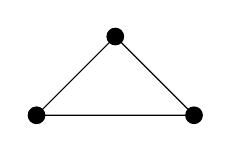
\begin{tikzpicture}
          \draw (0,0) -- (2,0) -- (1,1) -- (0,0);
          \filldraw (0,0) circle (3pt);
          \filldraw (2,0) circle (3pt);
          \filldraw (1,1) circle (3pt);
        \end{tikzpicture}
    \end{figure}

    \item Consider the following abstract simplicial complex 
    \begin{figure}[H]
      \centering
        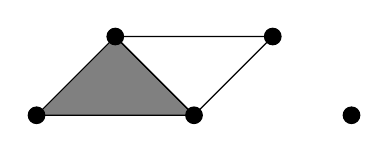
\begin{tikzpicture}
          \draw[fill=gray] (0,0) -- (2,0) -- (1,1) -- (0,0);
          \draw (2,0) -- (3,1) -- (1,1) -- (2,0);
          \filldraw (0,0) circle (3pt);
          \filldraw (2,0) circle (3pt);
          \filldraw (1,1) circle (3pt);
          \filldraw (3,1) circle (3pt);
          \filldraw (4,0) circle (3pt);
        \end{tikzpicture}
    \end{figure}
    It has the following faces \( \left\{ 1,2,4 \right\}, \left\{ 4,5 \right\}, \left\{ 2,5 \right\}, \left\{ 3 \right\} \).

    \item Consider the following triangulation 
    \begin{figure}[H]
      \centering
        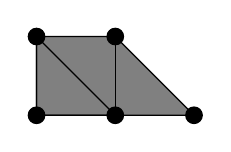
\begin{tikzpicture}
          \draw[fill=gray] (0,0) -- (1,0) -- (2,0) -- (1,1) -- (0,1) -- (0,0);
          \draw (0,0) -- (1,0) -- (0,1) -- (0,0);
          \draw (1,0) -- (1,1);
          \filldraw (0,0) circle (3pt);
          \filldraw (1,0) circle (3pt);
          \filldraw (1,1) circle (3pt);
          \filldraw (0,1) circle (3pt);
          \filldraw (2,0) circle (3pt);
        \end{tikzpicture}
    \end{figure}
    It has maximal cells \( \left\{ 1,2,4 \right\}, \left\{ 2,4,5 \right\}, \left\{ 2,3,5 \right\} \).

    \item Given a point configuration \( A = (a_1, \dots, a_5) \) and \( \omega = (1, 0,0,0, 1) \), we obtain a regular triangulation  
    \begin{figure}[H]
      \centering
        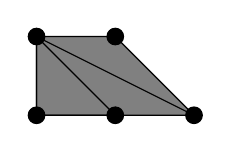
\begin{tikzpicture}
          \draw[fill=gray] (0,0) -- (1,0) -- (2,0) -- (1,1) -- (0,1) -- (0,0);
          \draw (0,0) -- (1,0) -- (0,1) -- (0,0);
          \draw (0,1) -- (2,0);
          \filldraw (0,0) circle (3pt);
          \filldraw (1,0) circle (3pt);
          \filldraw (1,1) circle (3pt);
          \filldraw (0,1) circle (3pt);
          \filldraw (2,0) circle (3pt);
        \end{tikzpicture}
    \end{figure}

    \item The twisted cube is given by \( A = \begin{bmatrix}
      3 & 2 & 1 & 0 \\ 0 & 1 & 2& 3
    \end{bmatrix} \). Consider the point configuration given by \( A \):
    \begin{figure}[H]
      \centering
        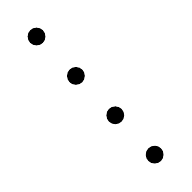
\begin{tikzpicture}
          \filldraw (1.5,0) circle (3pt);
          \filldraw (1,0.5) circle (3pt);
          \filldraw (0.5,1) circle (3pt);
          \filldraw (0,1.5) circle (3pt);
        \end{tikzpicture}
    \end{figure}
    It has 4 regular triangulations: 
    \begin{align*}
      \left\{ \left\{ 1,4 \right\} \right\}, \left\{  \left\{ 1,2 \right\}, \left\{ 2,3 \right\}, \left\{ 3,4 \right\}\right\}, \left\{ \left\{ 1,3 \right\}, \left\{ 3,4 \right\} \right\}, \left\{ \left\{ 1,2 \right\}, \left\{ 2,4 \right\} \right\} .
    \end{align*}
    \( \left\{ \left\{ 1,3 \right\}, \left\{ 2,4 \right\} \right\} \) is not a \emph{regular} triangulation.
  \end{itemize}
\end{eg}

\marginnote{\small{Lec19 04/07/23}}

\begin{defi}[Associated abstract simplicial complex]\index{associated abstract simplicial complex}
  Let \( A = \left\{ \mathbf a_1, \dots,\mathbf  a_n \right\} \subset \mathbb Z^d \) be a point configuration. Let \( \omega \in \mathbb R^n_{\geq 0} \). This induces a regular triangulation of \( A \). To this regular triangulation we associate an abstract simplicial complex \( \Delta_\omega(A) \) that consists of faces \( \sigma \in 2^{[n]} \) that correspond to faces seen from below of the lifted point configuration. Algebraically, the \textbf{associated abstract simplicial complex} is defined as 
  \begin{align*}
    \Delta_\omega(A) &=  \left\{ \sigma \in 2^{[n]} : \exists \mathbf c \in \mathbb R^d \text{ with } \begin{bmatrix}\mathbf c\\-1\end{bmatrix}\cdot \begin{bmatrix}\mathbf a_i\\w_i\end{bmatrix}  = 0, \begin{bmatrix}\mathbf c\\-1\end{bmatrix}\cdot \begin{bmatrix}\mathbf a_j\\w_j\end{bmatrix}  < 0,  \forall i \in \sigma, \forall j \notin \sigma \right\} \\
    &= \left\{ \sigma \in 2^{[n]} : \exists \mathbf  c \in \mathbb R^d \text{ with } \mathbf c \mathbf a_i = w_i, \mathbf c \mathbf a_j < w_j, \forall i \in \sigma, \forall j \notin \sigma \right\}
  \end{align*}
\end{defi}

\begin{defi}[Initial complex]\index{initial complex}
  Let \( \prec \) be a monomial order. The \textbf{initial (abstract simplicial) complex} of a toric ideal \( I_A \) is defined as 
  \begin{align*}
    \Delta_\prec(I_A) = \left\{ 
      \sigma \in 2^{[n]} : \not \exists f \in I_A \text{ with } \mathrm{supp}(\mathrm{in}_\prec(f)) = \sigma
     \right\}.
  \end{align*}
\end{defi}

\begin{prop}
  \( \Delta_\prec(I_A) \) is indeed an abstract simplicial complex.
\end{prop}

\begin{proof}
  We prove the claim by contraposition.   Assume \( \sigma \in \Delta_\prec(I_A) \) is a face and \( F \subset \sigma \). Assume that there is some \( f \in I_A \) such that \( \mathrm{supp}(\mathrm{in}_\prec(f)) = F \). Define \( \alpha = \sigma \setminus F \). Then \( \mathrm{supp}(\mathrm{in}_\prec(x^\alpha \cdot f)) = \sigma \) and \( x^\alpha \cdot f \in I_A \).
\end{proof}

Our goal is to prove \textbf{Sturmfels Theorem} (1991): if \( \omega \) represents \( \mathrm{in}_\prec(I_A) \), then 
\begin{align*}
  \Delta_\prec(I_A) = \Delta_\omega(A).
\end{align*}

\begin{defi}[Stanley-Reisner ideal]
  Let \( \Delta \subset 2^{[n]} \) be an abstract simplicial complex. The \textbf{Stanley-Reisner ideal}\index{Stanley-Reisner ideal} \( I(\Delta) \) of \( \Delta \) is 
  \begin{align*}
    I(\Delta) = \left( \prod_{i \in \sigma} x_i : \sigma \notin \Delta \right) \subset k [x_1, \dots, x_n].
  \end{align*}
  The Stanley-Reisner ideal is a squarefree monomial ideal, i.e. it has squarefree monomial generators. A monomial \( x^\alpha \) is called squarefree if \( \alpha_i \in \left\{ 0,1 \right\} \) for all \( i=1, \dots, n \).
\end{defi}

\begin{remark}
  The Stanley-Reisner ideal is generated by the \emph{minimal non-faces of \( \Delta \)}.
\end{remark}

\begin{eg}\(  \)
\begin{itemize}
  \item \( I(2^{[n]}) = 0 \)
  \item \( I(\emptyset) = (1) \)
  \item ...
\end{itemize}
\end{eg}

\begin{remark}[Stanley-Reisner complex]\index{Stanley-Reisner complex}
  We defined the following map:
  \begin{align*}
    \left\{ \text{abstract simplicial complex in \( [n] \)} \right\} &\to \left\{ \text{squarefree monomials in \( k[x_1, \dots, x_n] \)} \right\}\\
    \Delta &\mapsto I(\Delta)
  \end{align*}
  This is even a bijection with an inverse given by 
  \begin{align*}
    \Delta(I) = \left\{ \sigma \in 2^{[n]} : \prod_{i \in \sigma} x_i \notin I  \right\}
  \end{align*}
  for a squarefree ideal \( I \). 
  \( \Delta(I) \) is called the \textbf{Stanley-Reisner complex}.
\end{remark}

\subsection{Sturmfels theorem}

Note that the radical of a monomial ideal is squarefree. Square free ideals are radical.

\begin{prop}
  Let \( \prec \) be a monomial order and let \( I_A \) be a toric ideal. Then 
  \begin{align*}
    \Delta_\prec(I_A) = \Delta(\sqrt{\mathrm{in}_\prec(I_A)}).
  \end{align*}
\end{prop}

\begin{proof}\(  \)
  \begin{itemize}
    \item \( \subset \): Contraposition. Take \( \sigma \notin \Delta(\sqrt{\mathrm{in}_\prec(I_A)}) \). This means that \( \prod_{i \in \sigma} x_i^m \in {\mathrm{in}_\prec(I_A)} \) for some \( m \in \mathbb N \). So there exists \( f \in I_A \) such that \( \mathrm{in}_\prec(f) = \prod_{i \in \sigma} x_i^m \). In particular, \( \mathrm{supp}(\mathrm{in}_\prec(f)) = \sigma \). Hence, \( \sigma \notin \Delta_\prec(I_A) \).
    \item \( \supset \): Contraposition. Let \( \sigma \notin \Delta_{\prec}(I_A) \). So there is some \( f \in I_A \) such that \( \mathrm{supp}(\mathrm{in}_\prec(f)) = \sigma \). Thus, \( \mathrm{in}_\prec(f) = \prod_{i \in \sigma} x_i^{\alpha_i} \). Then, \( \prod_{i \in \sigma} x_i^m  \in \mathrm{in}_\prec(I_A)\) for \( m = \max \alpha_i \).
  \end{itemize}
\end{proof}

\begin{mdframed}
\begin{thm}[Sturmfels 1991]\index{Sturmfels theorem}
  If \( \omega \in \mathbb R^n_{\geq 0} \) represents \( \mathrm{in}_\prec(I_A) \), then 
  \begin{align*}
    \Delta_\prec(I_A) = \Delta_\omega(A).
  \end{align*}
\end{thm}
\end{mdframed}

\begin{proof}
It suffices to prove 
\begin{align*}
  I(\Delta_\omega(A)) = \sqrt{\mathrm{in}_\omega(I_A)}
\end{align*}
for generic \( \omega \). Applying \( \Delta(\bullet) \) yields 
\begin{align*}
  \Delta_\omega(A) = \Delta(\sqrt{\mathrm{in}_\omega(I_A)}) = \Delta(\sqrt{\mathrm{in}_\prec(A)}) = \Delta_\prec(I_A).
\end{align*}
Let's prove \(   I(\Delta_\omega(A)) = \sqrt{\mathrm{in}_\omega(I_A)}\).

\begin{itemize}
  \item \( \subset \): Let \( \sigma \notin \Delta_\omega(A) \), \( k = |\sigma| \). This means that \( \sigma \) does not define a lower face of a regular triangulation induced by \( \omega \). So there is no \( \mathbf c \in \mathbb R^d \) suc that \( \mathbf c \mathbf a_i = \omega_i \) and \( \mathbf c \mathbf a_j < \omega_j \) for all \( i \in \sigma \) and \( j \notin \sigma \)...
  \item \( \supset \): carefully trace the proof back 
\end{itemize}
\end{proof}

\marginnote{\small{Lec20 11/07/23}}

\begin{eg}
  Let \( A = \begin{bmatrix}
    1 & 1 & 1& 1& 1& 1 \\
    0 & 1 & 2 & 0 & 1 & 0 \\
    0 & 0 & 0 & 1 & 1 & 2
  \end{bmatrix} \in \mathbb Z^{3 \times 6} \). Here is the point configuration \( A \) cut at \( x = 1 \):
  \begin{figure}[H]
    \centering
      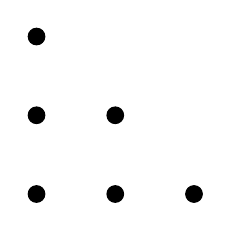
\begin{tikzpicture}
        % \draw (0,0) -- (1,0) -- (2,0) -- (1,1) -- (0,2) -- (0,1) -- (0,0);
        \filldraw (0,0) circle (3pt);
        \filldraw (1,0) circle (3pt);
        \filldraw (2,0) circle (3pt);
        \filldraw (0,1) circle (3pt);
        \filldraw (1,1) circle (3pt);
        \filldraw (0,2) circle (3pt);
      \end{tikzpicture}
  \end{figure}
  A toric ideal is given by 
  \begin{align*}
    I_A = (ac - b^2, ae - bd, af - d^2, cd -be, ef - e^2, de -bf).
  \end{align*}
  Here is regular triangulation induced by \( \omega = (10, 1, 10, 5, 1, 1) \):
  \begin{figure}[H]
    \centering
      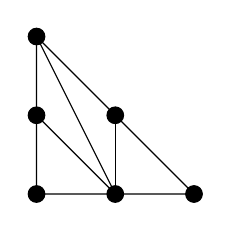
\begin{tikzpicture}
        \draw (0,0) -- (1,0) -- (2,0) -- (1,1) -- (0,2) -- (0,1) -- (0,0);
        \draw (0,1) -- (1,0);
        \draw (1,0) -- (1,1);
        \draw (0,2) -- (1,0);
        \filldraw (0,0) circle (3pt);
        \filldraw (1,0) circle (3pt);
        \filldraw (2,0) circle (3pt);
        \filldraw (0,1) circle (3pt);
        \filldraw (1,1) circle (3pt);
        \filldraw (0,2) circle (3pt);
      \end{tikzpicture}
  \end{figure}
  This triangulation is unimodular. We compute \( \mathrm{in}_\omega(I_A) =\sqrt{\mathrm{in}_\omega(I_A)} = (ac, ae, af, cd, cf, de) \). We claim (without proof):
  \begin{align*}
    \mathrm{in}_\omega(I_A) \text{ is squarefree} \iff \Delta_\omega \text{ is unimodular}
  \end{align*}

  Here is a different triangulation:
  Given \( \omega' = (1, 10, 1, 10, 10, 1) \) we obtain a non-unimodular triangulation. Moreover, we see that \( \mathrm{in}_{\omega'}(I_A) = (b^2, bd, d^2, be, e^2, de) \) is not squarefree.

  Note that \( \sqrt{\mathrm{in}_{\omega'}(I_A)} = (b,d,e) \). The triangulation \( \Delta_{\omega'}(A) \) has unique facet \( \left\{ a,c,f \right\} \). 
  \begin{figure}[H]
    \centering
      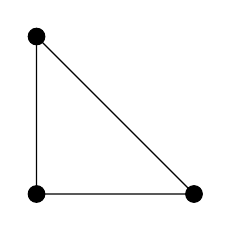
\begin{tikzpicture}
        \draw (0,0) -- (1,0) -- (2,0) -- (1,1) -- (0,2) -- (0,1) -- (0,0);
        \filldraw (0,0) circle (3pt);
        \filldraw (2,0) circle (3pt);
        \filldraw (0,2) circle (3pt);
      \end{tikzpicture}
  \end{figure}
  
  The Stanley-Reisner ideal yields \( I(\Delta_{\omega'}(A)) = (b,d,e) \). We see that the formula 
  \begin{align*}
    I(\Delta_{\omega'}(A)) = \sqrt{\mathrm{in}_{\omega'}(I_A)} 
  \end{align*}
  holds.
  
\end{eg}

\begin{eg}[Twisted cube]
Let \( A = \begin{bmatrix}
  1 & 1 & 1 & 1 \\ 0 & 1 & 2 & 3
\end{bmatrix} \). Using a computer we compute the Gröbner fan of \( I_A \). The Gröbner fan has 8 maximal cones that correspond to the following initial ideals 
\begin{enumerate}
  \item \( (bd,ad,ac) \)
  \item \( (ad,bd,b^2) \)
  \item \( (ad^2,bd,bc,b^2) \)
  \item \( (bd,b^2,bc,c^3) \)
  \item \( (ad,ac,c^2) \)
  \item \( (a^2d,ac,c^2,bc) \)
  \item \( (ac,c^2,bc,b^3) \)
  \item \( (c^2,bc,b^2) \)
\end{enumerate}
We can draw the Gröbner fan embedded in its 2-dimensional linearity space 
\begin{figure}[H]
  \centering
  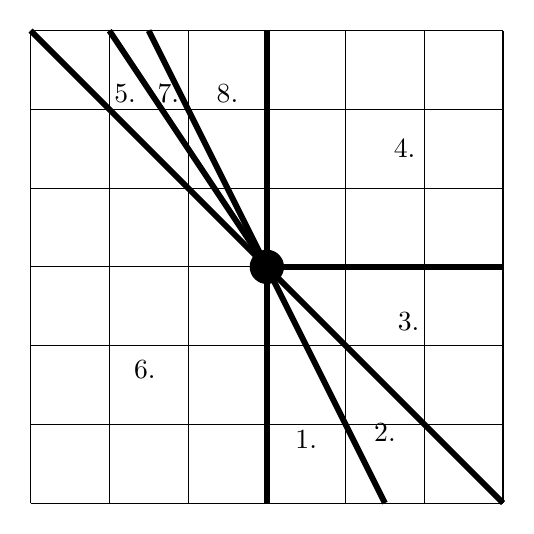
\begin{tikzpicture}
    \draw[step=1.0,black,thin] (-3,-3) grid (3,3);
    \draw [line width=0.75mm] (0,0) -- (0,3);
    \draw [line width=0.75mm] (0,0) -- (-2,3);
    \draw [line width=0.75mm] (0,0) -- (-1.5,3);
    \draw [line width=0.75mm] (0,0) -- (3,0);
    \draw [line width=0.75mm] (0,0) -- (-3,3);
    \draw [line width=0.75mm] (0,0) -- (3,-3);
    \draw [line width=0.75mm] (0,0) -- (0,-3);
    \draw [line width=0.75mm] (0,0) -- (1.5,-3);
    \draw (1.75,1.5) node {\( 4. \)};
    \draw (1.8,-0.7) node {\(3. \)};
    \draw (1.5,-2.1) node {\(2. \)};
    \draw (0.5,-2.2) node {\(1. \)};
    \draw (-1.8,2.2) node {\(5. \)};
    \draw (-1.25,2.2) node {\(7. \)};
    \draw (-0.5,2.2) node {\(8. \)};
    \draw (-1.55,-1.3) node {\(6. \)};
    \filldraw (0,0) circle (6pt);
  \end{tikzpicture}
  \caption{Gröbner fan embedded in its linearity space}
\end{figure}
If we take the radical ideals of the 8 distinct initial ideals, we obtain 4 distinct radical ideals: \( (bd, ad, ac), (ad,b), (b,c), (c,ad) \). Since we have \(  I(\Delta_\omega(A)) = \sqrt{\mathrm{in}_\omega(I_A)}\), there must exist 4 regular triangulations of \( A \). Each regular triangulation corresponds to squarefree monomial ideals.
\begin{figure}[H]
  \centering
  \begin{subfigure}[b]{0.2\linewidth}
    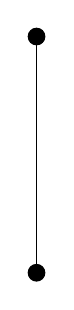
\begin{tikzpicture}
      \draw (1,0) -- (1,3);
      \filldraw (1,0) circle (3pt);
      \filldraw (1,3) circle (3pt);
    \end{tikzpicture}
    \caption*{\( (b,c) \)}
  \end{subfigure}
  \begin{subfigure}[b]{0.2\linewidth}
    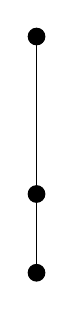
\begin{tikzpicture}
      \draw (1,0) -- (1,3);
      \filldraw (1,0) circle (3pt);
      \filldraw (1,1) circle (3pt);
      \filldraw (1,3) circle (3pt);
    \end{tikzpicture}
    \caption*{\( (ad,b) \)}
  \end{subfigure}
  \begin{subfigure}[b]{0.2\linewidth}
    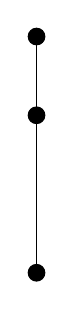
\begin{tikzpicture}
      \draw (1,0) -- (1,3);
      \filldraw (1,0) circle (3pt);
      \filldraw (1,2) circle (3pt);
      \filldraw (1,3) circle (3pt);
    \end{tikzpicture}
    \caption*{\( (ad,c) \)}
  \end{subfigure}
  \begin{subfigure}[b]{0.2\linewidth}
    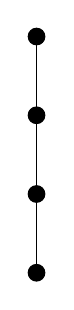
\begin{tikzpicture}
      \draw (0,0) -- (0,3);
      \filldraw (0,0) circle (3pt);
      \filldraw (0,1) circle (3pt);
      \filldraw (0,2) circle (3pt);
      \filldraw (0,3) circle (3pt);
    \end{tikzpicture}
    \caption*{\( (ad,ac, bd) \)}
  \end{subfigure}
\end{figure}
Let's group together the weights that induce the same regular triangulation of \( A \).
\begin{figure}[H]
  \centering
  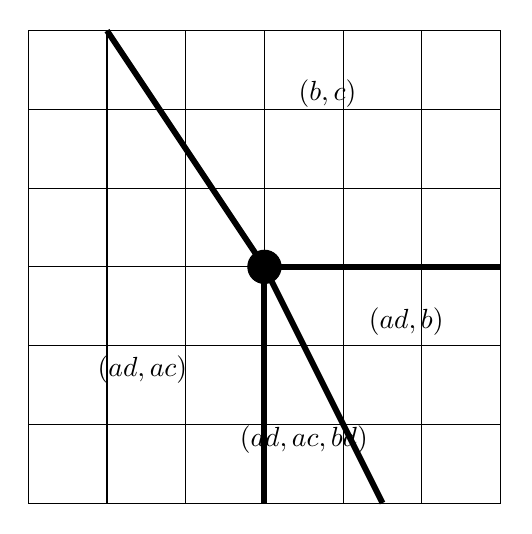
\begin{tikzpicture}
    \draw[step=1.0,black,thin] (-3,-3) grid (3,3);
    \draw [line width=0.75mm] (0,0) -- (3,0);
    \draw [line width=0.75mm] (0,0) -- (-2,3);
    \draw [line width=0.75mm] (0,0) -- (0,-3);
    \draw [line width=0.75mm] (0,0) -- (1.5,-3);
    \draw (1.8,-0.7) node {\( (ad,b) \)};
    \draw (0.5,-2.2) node {\( (ad,ac,bd) \)};
    \draw (0.8,2.2) node {\( (b,c) \)};
    \draw (-1.55,-1.3) node {\( (ad,ac) \)};
    \filldraw (0,0) circle (6pt);
  \end{tikzpicture}
  \caption{Secondary fan: Each maximal cone corresponds to a regular triangulation.}
\end{figure}
\end{eg}

\subsection{Secondary fan}

Let's define the secondary fan. Given \( A \in \mathbb Z^{d \times n} \), we define an equivalence relation 
\begin{align*}
  \omega \sim \omega ' \iff \Delta_\omega(A) = \Delta_{\omega'}(A)
\end{align*}
for \( \omega, \omega' \in \mathbb R^n \). By Sturmfels theorem, the equivalence class \( C_A[\omega]  \) consists of a union of Gröbner cones \( C_{I_A}[\omega] = \left\{ \omega ' \in \mathbb R^n : \mathrm{in}_\omega(I_A) = \mathrm{in}_\omega(I_A) \right\} \) with same radical initial ideal \( \sqrt{\mathrm{in}_\omega(I_A)} \), i.e.
\begin{align*}
  C_A[\omega] = \left\{ \omega ' \in \mathbb R^n : \sqrt{\mathrm{in}_\omega(I_A)} = \sqrt{\mathrm{in}_\omega(I_A)}  \right\}.
\end{align*}
There are adjacent cones in \( \mathrm{GFan}(I_A) \) because \( C_A[\omega] \) is convex.

\begin{prop}
  \( C_A[\omega] \) is convex.
\end{prop}

\begin{proof}
  Use the definition 
  \begin{align*}
    \Delta_\omega(A)  = \left\{ \sigma \in 2^{[n]} : \exists \mathbf  c \in \mathbb R^d \text{ with } \mathbf c \mathbf a_i = w_i, \mathbf c \mathbf a_j < w_j, \forall i \in \sigma, \forall j \notin \sigma \right\}
  \end{align*}
  and take two \( \sigma, \sigma' \in C_A[\omega] \). Show that \( \lambda\sigma + (1-\lambda) \sigma' \in C_A[\omega]\) which is easy to show.
\end{proof}

\begin{defi}[Secondary fan]
  The secondary fan\index{secondary fan} of \( A \in \mathbb Z^{d \times n} \) is the polyhedral fan \( S_A \) which has 
  \begin{align*}
    \left\{ \overline{C_A[\omega]} : \omega \in \mathbb R^n \right\} 
  \end{align*} as maximal cones.
\end{defi}

\begin{remark}
  Clearly, \( \omega \in \mathbb R^n \), \( C_I[\omega] \subset C_A[\omega
  ] \). Thus, the Gröbner fan of \( I_A \) is a refinement of \( S_A \).
\end{remark}

\begin{remark}
  Gel'fand, Kapranov,  Zelevinsky proved in 1994 that there exists a polytope \( \sum(A) \) such that \( \mathcal{N}(\sum(A)) = S_A \) if \( (1, \dots, 1) \in \mathrm{rowspan}(A) \) (this condition makes \( I_A \) homogeneous). This is called the \textbf{secondary polytope}\index{secondary polytope} of \( A \).
\end{remark}

\begin{remark}
  \( A \) is called unimodular if all triangulations of \( A \) are unimodular.

  If \( A \) is unimodular, then \( \mathrm{GFan}(I) = S_A \) and \( \mathrm{State}(I_A) = \sum(A) \).

  If \( A \) is unimodular, then \( C_A = \mathrm{Gr}(A) \).
\end{remark}

\clearpage
\section{Tropical Geometry}
See last two lecture notes uploaded on ISIS.


\clearpage
\section{Review}

\begin{itemize}
  \item What is a monomial order?
  \item How to characterize a well-order?
  \item When is a total order a well-order?
  \item Give examples of monomial orders
  \item State the multivariate division algorithm and prove the correctness
  \item What is Gröbner basis? What is a minimal Gröbner basis? A reduced Gröbner basis?
  \item Does a Gröbner basis always exist?
  \item Is the Gröbner basis really a basis?
  \item State the main theorem about Gröbner basis
  \item Does a reduced Gröbner basis always exist?
  \item Prove the uniqueness of the reduced Gröbner basis 
  \item State Buchberger's criterion and prove it
  \item State Buchberger's algorithm
  \item What are standard monomials?
  \item Prove Macaulay's Theorem
  \item Prove the two corollaries of Macaulay's Theorem
  \item Prove that every ideal has only finitely many distinct initial ideals
  \item Does a universal Gröbner basis always exist?
  \item \(     \mathrm{in}_{\prec_\omega} (I) = \mathrm{in}_\prec(\mathrm{in}_\omega(I))  \)
  \item Give a Gröbner basis of \( \mathrm{in}_\omega(I) \).
  \item Representation of initial ideals by weight vectors
  \item Explain the relationship between \( \mathrm{New}() \), \( \mathrm{in} \), \( \mathrm{face} \)
  \item \( C_I[\omega] \) is a polyhedral cone
  \item Explain the formula \( C_I[\omega] = N_P(\mathrm{face}_\omega(P)) \) with \( P = \mathrm{New}(\prod_{g \in \mathcal{G}} g) = \sum \mathrm{New}(g) \)
  \item Is the Gröbner fan really a fan?
  \item How to compute the Gröbner fan of a principal ideal?
  \item Can there be infinitely many Gröbner cones \( \overline{C_I[\omega]}? \)
  \item How to draw the Gröbner fan?
  \item Characterization of \( \omega \)-homogeneous ideals
  \item Gröbner region of homogeneous ideals
  \item Newton polytope and state polytope
  \item Existence of state polytope
  \item Give a formula for the state polytope
  \item What is a toric ideal?
  \item Is it prime? 
  \item Can a toric ideal contain a monomial?
  \item Explain the relationship between toric ideals and linear combinations of binomials
  \item How does the reduced Gröbner basis of a toric ideal look like?
  \item How to compute the Gröbner basis of a toric ideal?
  \item What is a Graver basis?
  \item What is the relationship between a Graver basis and a Gröbner basis?
  \item What is a rational polyhedral cone?
  \item What is a circuit?
  \item Relationship between circuits, Gröbner basis and primitive binomials
  \item Can we say something about the total degree of a primitive binomial?
  \item Let's move on to triangulations: What is an abstract simplicial complex?
  \item What is the associated abstract simplicial complex? 
  \item What is the initial complex?
  \item What is the Stanley-Reisner complex / ideal?
  \item What is Sturmfels theorem?
\end{itemize}


\appendix

\clearpage
\section{Appendix: Rings and ideals}

We assume that all rings are commutative and have \( 1 \).

\begin{defi}[Ideal]
  Let \( R \) be a ring. An \textbf{ideal} \( I \subset R \) is an additive subgroup that also satisfies 
  \( ab \in I, \; \forall b \in R, \forall a \in I \).
\end{defi}

\begin{defi}[Generating system]
  The ideal generated by \( A \subset R \) is defined as
  \begin{align*}
    (A) = \left\{ Ra_1 + \dots + Ra_n : a_i \in A, n \in \mathbb N \right\}
  \end{align*}
  It is the smallest ideal containing \( A \). A \textbf{principal ideal} \( I \) is an ideal generated by one element. We say an ideal is \textbf{finitely generated} if \( I = (A) \) for some finite \( A \). We call such \( A \) a \textbf{basis} of \( I \).
\end{defi}

\begin{remark}
  The ideal \( (\emptyset)  \) generated by the empty set is the zero ideal.
\end{remark}

\begin{remark}\(  \)
  \begin{enumerate}
    \item \( I + J = \left\{ a + b : a \in I, b \in J \right\} \) is an ideal
    \item \( I \cap J \) is an ideal
    \item Products of ideal need not be ideals, so we define \( IJ \) as the ideal generated by \( \left\{ ab : a \in I, b \in J \right\} \). It is always true that \( IJ \subset I \cap J \). The converse fails for \( I=J=(2) \subset \mathbb Z \).

  \end{enumerate}
\end{remark}

\begin{remark}
  An ideal \( I \subset R \) always contains \( 0 \).
\end{remark}

\begin{remark}
  An ideal \( I \subset R \) contains \( 1 \) if and only if \( I = R \). 
\end{remark}

\begin{thm}[Hilbert's Basis Theorem]
  Every ideal \( I \subset k[x_1,\dots,x_n] \) is finitely generated.
\end{thm}




\clearpage
\section{Appendix: Farkas Lemma}

\begin{prop}
  Given \( A \in \mathbb R^{d \times n} \) and \( b \in \mathbb R^d \), exactly one of the following holds 
  \begin{itemize}
    \item there exists \( x \in \mathbb R^n_{\geq 0 }  \) such that \( Ax = b \) or
    \item there exists \( c \in \mathbb R^d \) such that \( c^TA \geq 0 \) and \( c^Tb < 0 \).
  \end{itemize}
\end{prop}

\begin{prop}\label{farkas-2}
  Given \( A \in \mathbb R^{d \times n} \) and \( b \in \mathbb R^d \), exactly one of the following holds 
  \begin{itemize}
    \item there exists \( x \in \mathbb R^n_{\geq 0 }  \) such that \( Ax\leq= b \) or
    \item there exists \( c \in \mathbb R^d_{\geq 0} \) such that \( c^TA \geq 0 \) and \( c^Tb < 0 \).
  \end{itemize}
\end{prop}

\clearpage
\section{Appendix: Polyhedra, cones and fans}

We quickly summarize all important facts regarding polyhedra, cones and fans.

\begin{defi}[Convex cone]\index{cone!convex}
  A set \( C \subset \mathbb R^n \) is called a \textbf{convex cone} if for every \( x,y \in C \) and \( \lambda > 0 \) we have \( x+y \in C \) and \( \lambda x \in C \).
\end{defi}

\begin{defi}[Conic hull]\index{conic hull}
  Given vectors \( x_1,...,x_k \in \mathbb R^n \) the \textbf{conic hull} is defined to be the set that contains all vectors of the form 
  \begin{align*}
    \alpha x_1 + ... + \alpha_k x_k 
  \end{align*}
  where \( \alpha \geq 0 \).
\end{defi}

\begin{defi}[Face of a cone]
  A face of a cone \( C \) is of the form \( \mathrm{face}_{\omega}(C) = \left\{ x \in C: \omega x \geq \omega y, \, \forall y \in C \right\} \).
\end{defi}

\begin{defi}[Polyhedral cone]\index{cone!polyhedral}
  A cone is \textbf{polyhedral} if \( C = \mathrm{cone}(v_1,...,v_k) \). Equivalently by Minkowski-Weyl, a cone \( C \) is polyhedral if \( C \) is a polyhedron, that is, it is the intersection of a finite number of half-spaces, each containing \( 0 \) on their boundary.
\end{defi}

\begin{figure}[H]
  \centering
  \includegraphics[width=10cm]{assets/not-polyhedral-cone.png}
  \caption{A cone that is not polyhedral}
\end{figure}

\begin{defi}[Polyhedral fan]
  A polyhedral fan is a collection \( \mathcal{F} = \left\{ C_1,...,C_n \right\} \) of polyhedral cones such that 
  \begin{enumerate}
    \item every face of a cone in \( \mathcal{F} \) is also a cone in \( \mathcal{F} \), and 
    \item the intersection of any two cones in \( \mathcal{F} \) is a {common} face.
  \end{enumerate}
  The \textbf{support of a fan}\index{support of fan} is \( \bigcup C_i \). If the support of a fan is \( \mathbb R^n \) then we say that \( \mathcal{F} \) is \textbf{complete}\index{complete fan}.
\end{defi}

\begin{eg}[Normal fan]\index{normal fan}
  Let \( P \subset \mathbb R^n \) be a polytope. Its normal fan \( \mathcal{N}_P \) consists of normal cones\index{normal cone} \( \left\{ \mathcal{N}_P(F) : \text{\( F \neq \emptyset \) is a face of \( P \)} \right\} \) where \( \mathcal{N}_P(F) = \overline{\left\{ \omega \in \mathbb R^n : \mathrm{face}_\omega(P) = F \right\}} \).
\end{eg}

\printindex

\end{document}
